\documentclass[a4paper, 11pt, titlepage, twoside]{report}
\usepackage[a4paper]{geometry}
\usepackage{fancyhdr}
\usepackage{charter}
\usepackage{pstricks,pst-node,pst-text,pst-3d,pst-eucl}
\usepackage{psfrag}
\usepackage{import}
\usepackage{graphicx}
\usepackage{subfigure}
\usepackage{amssymb,amstext,amsfonts} %% ... with default font
\usepackage{amsmath}
\usepackage{mathrsfs}
%\usepackage{txfonts}
\usepackage{listings}
%\usepackage{tikz}
%\usetikzlibrary{shapes,arrows}
\usepackage{lmodern}
\usepackage{microtype}
\usepackage{nicefrac}
\usepackage[load=prefixed, load=abbr, alsoload=hep, alsoload=astro]{siunitx}
\renewcommand{\sfdefault}{lmss}
\renewcommand{\ttdefault}{lmtt}
\usepackage[T1]{fontenc}
\usepackage{braket}
\usepackage{slashed}
\usepackage{afterpage}
\usepackage[latin9]{inputenc}
\usepackage{fixmath}
\usepackage[numbers, sort&compress]{natbib}
\renewcommand{\bibfont}{\footnotesize}
\renewcommand{\bibname}{{R\lowercase{eferences}}}
\setlength{\bibhang}{0pt} 


  \hyphenpenalty=4000
  \tolerance=1000
  
\headheight 13.6pt
\textheight = 45\baselineskip

\def\today{\number\day\space\ifcase\month\or January\or February\or March\or April\or May\or June\or July\or August\or September\or October\or November\or December\fi\space\number\year}

\newcommand{\eqnref}[1]{equation~(\ref{eq:#1})}
\newcommand{\Eqnref}[1]{Equation~(\ref{eq:#1})}
\newcommand{\secref}[1]{section~\ref{sec:#1}}
\newcommand{\Secref}[1]{Section~\ref{sec:#1}}
\newcommand{\apref}[1]{appendix~\ref{sec:#1}}
\newcommand{\Apref}[1]{Appendix~\ref{sec:#1}}
\newcommand{\tabref}[1]{table~\ref{tab:#1}}
\newcommand{\Tabref}[1]{Table~\ref{tab:#1}}
\newcommand{\figref}[1]{figure~\ref{fig:#1}}
\newcommand{\Figref}[1]{Figure~\ref{fig:#1}}

\newcommand{\sinc}{{\rm sinc}}

\newcommand{\sub}[1]{\ensuremath{_\mathrm{#1}}}
\newcommand{\super}[1]{\ensuremath{^\mathrm{#1}}}

\newcommand{\recip}[1]{\ensuremath{\frac{1}{#1}}}
\newcommand{\nicerecip}[1]{\ensuremath{\nicefrac{1}{#1}}}

\newcommand{\order}[1]{\ensuremath{\mathcal{O}({#1})}}

\newcommand{\innerprod}[2]{\ensuremath{\left({#1}\middle|{#2}\right)}}

\newcommand{\Ibar}{{\declareslashed{}{\text{-}}{0.04}{0}{I}\slashed{I}}}
\newcommand{\lambdabar}{{\declareslashed{}{\text{--}}{0.04}{0}{\lambda}\slashed{\lambda}}}

% Define differential operators
\newcommand{\dd}{\ensuremath{\mathrm{d}}}
\newcommand{\diff}[2]{\ensuremath{\frac{\dd {#1}}{\dd {#2}}}}
\newcommand{\linediff}[2]{\ensuremath{\dd {#1}/\dd {#2}}}
\newcommand{\nicediff}[2]{\ensuremath{\nicefrac{\dd {#1}}{\dd {#2}}}}
\newcommand{\diffop}[1]{\ensuremath{\frac{\dd}{\dd {#1}}}}
\newcommand{\difftwo}[2]{\ensuremath{\frac{\dd^2 {#1}}{\dd {#2}^2}}}
\newcommand{\linedifftwo}[2]{\ensuremath{\dd^2 {#1}/\dd {#2}^2}}
\newcommand{\nicedifftwo}[2]{\ensuremath{\nicefrac{\dd^2 {#1}}{\dd {#2}^2}}}
\newcommand{\difftwoop}[1]{\ensuremath{\frac{\dd^2}{\dd {#1}^2}}}
\newcommand{\diffn}[3]{\ensuremath{\frac{\dd^{#3} {#1}}{\dd {#2}^{#3}}}}
\newcommand{\linediffn}[3]{\ensuremath{\dd^{#3} {#1}/\dd {#2}^{#3}}}
\newcommand{\nicediffn}[3]{\ensuremath{\nicefrac{\dd^{#3} {#1}}{\dd {#2}^{#3}}}}
\newcommand{\diffnop}[2]{\ensuremath{\frac{\dd^{#2}}{\dd {#1}^{#2}}}}
\newcommand{\partialdiff}[2]{\ensuremath{\frac{\partial {#1}}{\partial {#2}}}}
\newcommand{\linepartialdiff}[2]{\ensuremath{\partial {#1}/\partial {#2}}}
\newcommand{\nicepartialdiff}[2]{\ensuremath{\nicefrac{\partial {#1}}{\partial {#2}}}}
\newcommand{\partialdiffop}[1]{\ensuremath{\frac{\partial}{\partial {#1}}}}
\newcommand{\grad}{\ensuremath{\boldsymbol{\nabla}}}
\newcommand{\intd}[4]{\ensuremath{\int_{#1}^{#2}{#3}\,\dd{#4}}}

\begin{document}

\bibpunct{[}{]}{,\,}{s}{}{}

\pagestyle{fancy}
\renewcommand{\chaptermark}[1]{
\markboth{\chaptername
\ \thechapter.\ #1}{}}
\renewcommand{\sectionmark}[1]{\markright{\thesection\ #1}}
\fancyhf{}
\fancyhead[LE]{\leftmark}
\fancyhead[RE]{Christopher Berry}
\fancyhead[LO]{Exploring Strong Field Gravity}
\fancyhead[RO]{\rightmark}
\fancyfoot{}
\renewcommand{\footrulewidth}{0.1ex}
\fancyfoot[LO]{\today}
\fancyfoot[RE]{CPGS}
\fancyfoot[RO, LE]{\thepage}
\fancypagestyle{plain}{
\fancyhf{}
\renewcommand{\headrulewidth}{0pt}
\fancyfoot{}
\renewcommand{\footrulewidth}{0.1ex}
\fancyfoot[LO]{\today}
\fancyfoot[RE]{CPGS}
\fancyfoot[RO, LE]{\thepage}}
\renewcommand\floatpagefraction{.6}
\renewcommand\topfraction{.8}
\renewcommand\bottomfraction{.8}
\renewcommand\textfraction{.2}

\title{{\huge{}Exploring Strong Field Gravity}}
\author{{\Large{}Christopher Berry}\vspace{3mm}\\Churchill College\vspace{0.5mm}\\and\vspace{0.5mm}\\Institute of Astronomy,\vspace{0.5mm}\\University of Cambridge\vspace{5mm}\\{\Large{}Supervisor: Jonathan Gair}\vspace{5mm}}
\date{\includegraphics[width=0.25\textwidth]{../shield.eps}\vspace{11mm}\\{\LARGE{}Certificate of Postgraduate Study}\vspace{5mm}\\\today}
\maketitle

\begin{abstract}
This is exceedingly abstract
\end{abstract}

\chapter{Introduction}\setcounter{page}{1}

\section{Gravitation}

Detecting gravitational waves (GWs) would allow us to probe gravitational interactions in regimes that are currently inaccessible using more traditional, electromagnetic observations. For example, encounters between compact objects, like black holes or neutron stars, create gravitational fields that are both intensely strong and highly dynamical, a domain where GR has yet to be tested.

\section{Structure}

In chapter 2 we examine an alternate theory of gravity: metric $f(R)$. We focus on the modifications to gravitational radiation and possible observational tests that may be used to constrain the theory. Many of the results are already known in the literature, but are worked out here {\it ab initio}. We include them as a compendium of useful results, within a consistent system of notation, and to highlight some important points. Seemingly new results are found in sections \ref{sec:EM_tensor} and \ref{sec:Epicycle}.

In chapter 3 we investigate what might be inferred by observing gravitational radiation from an object on a highly eccentric orbit about the galactic centre. Waveform construction, signal analysis and parameter estimation are discussed, and some preliminary results are presented.

Finally in chapter 4 we outline further areas of interest that may be studied in the future.

\section{Conventions}

Throughout this work we will use the time-like sign convention of Landau and Lifshitz\cite{Landau1975}:
\begin{enumerate}
\item The metric has signature $(+,-,-,-)$.
\item The Reinann tensor is defined as ${R^\mu}_{\nu\sigma\rho} = \partial_\sigma {\Gamma^\mu}_{\nu\rho} - \partial_\rho {\Gamma^\mu}_{\nu\sigma} + {\Gamma^\mu}_{\lambda\sigma}{\Gamma^\lambda}_{\rho\nu} - {\Gamma^\mu}_{\lambda\rho}{\Gamma^\lambda}_{\sigma\nu}$.
\item The Ricci tensor is defined as the contraction $R_{\mu\nu} = {R^\lambda}_{\mu\lambda\nu}$.
\end{enumerate}
Greek indices are used to represent spacetime indices $\mu = \{0,1,2,3\}$ and lowercase Latin indices from the middle of the alphabet are used for spatial indices $i = \{1,2,3\}$. Uppercase Latin indices from the beginning of the alphabet will be used for the output of two LISA detector arms $A = \{\mathrm{I}, \mathrm{II}\}$, and lowercase Latin indices from the beginning of the alphabet are used for parameter space. Summation over repeated indices is assumed unless explicitly noted otherwise. Geometric units with $G = c = 1$ will be used where noted, but in general factors of $G$ and $c$ will be retained.

\chapter{Gravitational Radiation In $f(R)$ Theory}

\section{Introduction To $f(R)$ Theory}

General relativity (GR) is a well tested theory of gravity\cite{Will2006}; however it is still interesting to explore alternative theories. This may be motivated by the need to explain dark matter and dark matter in cosmology, trying to formulate a quantizable theory of gravity or simple curiosity regarding the uniqueness of GR. One of the simplest extensions to standard GR is the class of $f(R)$ theories\cite{Sotiriou2010, DeFelice2010}.

\subsection{The Action \& Field Equations}\label{sec:Action}

General relativity may be derived from the Einstein-Hilbert action\cite{Misner1973, Landau1975}
\begin{equation}
S\sub{EH}[g] = \frac{c^4}{16\pi G}\intd{}{}{R\sqrt{-g}}{^4x}.
\end{equation}
In $f(R)$ theory we make a simple modification of the action to include an arbitrary function of the Ricci scalar $R$ such that\cite{Buchdahl1970}
\begin{equation}
S[g] = \frac{c^4}{16\pi G}\intd{}{}{f(R)\sqrt{-g}}{^4x}.
\end{equation}
Including the function $f(R)$ gives extra freedom in defining the behaviour of gravity; while this action may not encode the true theory of gravity it may at least contain sufficient information to act as an effective field theory, correctly describing phenomological behaviour\cite{Park2010}. We will assume that $f(R)$ is analytic about $R = 0$ so that it may be expressed as a power series\cite{Buchdahl1970, Psaltis2008}
\begin{equation}
f(R) = a_0 + a_1 R + \frac{a_2}{2!}R^2 + \frac{a_3}{3!}R^3 + \ldots
\end{equation}
Note that since the dimensions of $f(R)$ must be the same as of $R$, $[a_n] = [R]^{(1-n)}$. To link to GR we will set $a_1 = 1$; any rescaling may be absorbed into the definition of $G$.

The field equations are obtained by a variational principle; there are a number of choices for achieving this. To derive the Einstein field equations from the Einstein-Hilbert action one may use the standard metric variation or the Palatini variation\cite{Misner1973}. Both approaches may be used for $f(R)$, however they now yield different results\cite{Sotiriou2010, DeFelice2010}. Following the metric (or second order) formalism, one varies the action with respect to the metric $g^{\mu\nu}$, the resulting field equations being those for metric $f(R)$ gravity. Following the Palantini (or first order) formalism one varies the action with respect both to the metric $g^{\mu\nu}$ and to the connection ${\Gamma^\rho}_{\mu\nu}$, which are treated as independent quantities: the connection is not the Levi-Cevita metric connection.\footnote{Imposing that the metric and Palantini formalisms produce the same field equations, assuming an action that only depends on the metric and Reimann tensor, results in Lovelock gravity\cite{Exirifard2008}. Lovelock gravities require the field equations to be divergence free and no more than second order; in four dimensions the only possible Lovelock gravity is GR with a potentially non-zero cosmological constant\cite{Lovelock1970, Lovelock1971, Lovelock1972}.}

Finally, there is a third version of $f(R)$ gravity: metric-affine $f(R)$ gravity\cite{Sotiriou2007, Sotiriou2007b}. This goes beyond the Palantini formalism by supposing that the matter action is dependent on the variational independent connection. Parallel transport and the covariant derivative are divorced from the metric. This theory has its attractions: it allows for a natural introduction or torsion. However, it is not a metric theory of gravity and so cannot satisfy all the postulates of the Einstein equivalence principle\cite{Will2006}: a free particle does not necessarily follow a geodesic and so the effects of gravity may not be locally removed\cite{Exirifard2008}. The implications of this have not been fully explored, but for this reason we shall not consider the theory further.

We shall restrict our attention to consider only metric $f(R)$ gravity. The metric formalism is preferred as the Palantini formalism has undesirable properties: static spherically symmetric objects described by a polytropic equation of state are subject to a curvature singularity\cite{Barausse2008b, Barausse2008a}. Varying the action with respect to the metric $g^{\mu\nu}$ produces
\begin{equation}
\delta S = \frac{c^4}{16\pi G}\intd{}{}{\left\{f'(R)\sqrt{-g}\left[R_{\mu\nu} - \nabla_\mu\nabla_\nu\ + g_{\mu\nu}\Box\right] - f(R)\frac{1}{2\sqrt{-g}}gg_{\mu\nu}\right\}\delta g^{\mu\nu}}{^4x},
\end{equation}
where $\Box = g^{\mu\nu}\nabla_\mu\nabla_\nu$ is the d'Alembertian and a prime denotes differentiation with respect to $R$. Proceeding from here requires certain assumptions regarding surface terms. In the case of the Einstein-Hilbert action the surface terms gather into a total derivative. It is possible to subtract this from the action to obtain a well-defined variational quantity\cite{York1972, Gibbons1977}. However, this is not the case for general $f(R)$\cite{Madsen1989}. It is argued that since the action includes higher order derivatives of the metric we are at liberty to fix more degrees of freedom at the boundary, in so doing eliminating the importance of the surface terms\cite{Dyer2009a, Sotiriou2010}. There is no well described prescription for this so we proceed directly to the field equations.

The vacuum field equation is
\begin{equation}
f'R_{\mu\nu} - \nabla_\mu\nabla_\nu f' + g_{\mu\nu}\Box f' - \frac{f}{2}g_{\mu\nu} = 0.
\label{eq:Field_eq}
\end{equation}
For standard GR, when $f(R) = R$, this reduces to the familiar
\begin{equation}
R_{\mu\nu} - \frac{R}{2}g_{\mu\nu} = 0.
\end{equation}
Taking the trace of our field equation gives
\begin{equation}
f'R + 3\Box f' - 2f = 0.
\label{eq:Trace_eq}
\end{equation}
Note if we consider a uniform flat spacetime $R = 0$, this equation gives
\begin{equation}
a_0 = 0.
\label{eq:a_0}
\end{equation}
In analogy to the Einstein tensor, we shall define
\begin{equation}
\mathcal{G}_{\mu\nu} = f'R_{\mu\nu} - \nabla_\mu\nabla_\nu f' + g_{\mu\nu}\Box f' - \frac{f}{2}g_{\mu\nu},
\label{eq:G_tensor}
\end{equation}
so that in a vacuum
\begin{equation}
\mathcal{G}_{\mu\nu} = 0.
\end{equation}

\subsection{Conservation Of Energy-Momentum}

If we introduce matter with a stress-energy tensor $T_{\mu\nu}$, the field equation becomes
\begin{equation}
\mathcal{G}_{\mu\nu} = \frac{8\pi G}{c^4}T_{\mu\nu}.
\end{equation}
If we act upon this with the covariant derivative we obtain
\begin{align}
\frac{8\pi G}{c^4}\nabla^\mu T_{\mu\nu} = {} & \nabla^\mu\mathcal{G}_{\mu\nu} \nonumber \\
= {} & R_{\mu\nu}\nabla^\mu f' + f'\nabla^\mu\left(R_{\mu\nu} - \recip{2}R g_{\mu\nu}\right) - \left(\Box\nabla_\nu - \nabla_\nu\Box\right)f'.
\end{align}
The second term contains the covariant derivative of the Einstein tensor and so is zero. After some manipulation the final term can be shown to be
\begin{align}
\left(\Box\nabla_\nu - \nabla_\nu\Box\right)f' = {} & g^{\mu\sigma}\left[\nabla_\mu\nabla_\sigma\nabla_\nu - \nabla_\nu\nabla_\mu\nabla_\sigma\right]f' \nonumber \\
 = {} & R_{\tau\nu}\nabla^\tau f',
\end{align}
which is a useful geometric identity\cite{Koivisto2006a}. Using this we find that
\begin{align}
\frac{8\pi G}{c^4}\nabla^\mu T_{\mu\nu} = {} & R_{\mu\nu}\nabla^\mu f' - R_{\mu\nu}\nabla^\mu f' \nonumber \\
 = {} & 0.
\end{align}
Consequently we see that energy-momentum is a conserved quantity in the same way as in GR, as may be expected from the symmetries of the action.

\section{Linearized Theory}\label{sec:Lin}

We will now consider the case that the metric is perturbed slightly from flat Minkowski such that
\begin{equation}
g_{\mu\nu} = \eta_{\mu\nu} + h_{\mu\nu};
\end{equation}
where, more formally, we mean that $h_{\mu\nu} = \varepsilon H_{\mu\nu}$ for small parameter $\varepsilon$.\footnote{It is because we wish to perturb about flat spacetime that we have required $f(R)$ to be analytic about $R = 0$.} We will consider terms only to $\order{\varepsilon}$. Thus, the inverse metric is
\begin{equation}
g^{\mu\nu} = \eta^{\mu\nu} - h^{\mu\nu},
\end{equation}
where we have used the Minkowski metric to raise the indices on the right side, effectively defining
\begin{equation}
h^{\mu\nu} = \eta^{\mu\sigma}\eta^{\nu\rho}h_{\sigma\rho}.
\end{equation}
Similarly, the trace $h$ is given by
\begin{equation}
h = \eta^{\mu\nu}h_{\mu\nu}.
\end{equation}
This means that all quantities denoted by ``$h$'' are strictly $\order{\varepsilon}$. We will have to be careful later on to distinguish between quantities where the Minkowski metric has been used to raise indices and those where the full metric has been used.

The linearized ($\order{\varepsilon}$) connection coefficient is
\begin{equation}
{{\Gamma^{(1)}}^\rho}_{\mu\nu} = \frac{1}{2}\eta^{\rho\lambda}(\partial_\mu h_{\lambda\nu} + \partial_\nu h_{\lambda\mu} - \partial_\lambda h_{\mu\nu}).
\label{eq:Lin_Gamma}
\end{equation}
The covariant derivative of any perturbed quantity will be the same as the partial derivative to first order. The Riemann tensor is
\begin{equation}
{{R^{(1)}}^\lambda}_{\mu\nu\rho} = \frac{1}{2}(\partial_\mu\partial_\nu h^\lambda_\rho + \partial^\lambda\partial_\rho h_{\mu\nu} - \partial_\mu\partial_\rho h^\lambda_\nu - \partial^\lambda\partial_\nu h_{\mu\rho}),
\label{eq:Lin_Riemann}
\end{equation}
where we have raised the index on the differential operator with the background Minkowski metric. Contracting gives the Ricci tensor
\begin{equation}
{R^{(1)}}_{\mu\nu} = \frac{1}{2}(\partial_\mu\partial_\rho h^\rho_\nu + \partial_\nu\partial_\rho h^\rho_\mu -\Box h_{\mu\nu} - \partial_\mu\partial_\nu h),
\label{eq:Ricci}
\end{equation}
where the d'Alembertian operator is $\Box = \eta^{\mu\nu}\partial_\mu\partial_\nu$. Contracting this with $\eta^{\mu\nu}$ we find the first order Ricci scalar
\begin{equation}
R^{(1)} = \partial_\mu\partial_\rho h^{\rho\mu} - \Box h.
\label{eq:Scalar}
\end{equation}

Since $R^{(1)}$ is $\order{\varepsilon}$ we may write $f(R)$ as a Maclaurin series to first order such that
\begin{align}
f(R) = {} & a_0 + R^{(1)}\\
f'(R) = {} & 1 + a_2 R^{(1)}.
\end{align}
As we are perturbing from a flat Minkowski background where the Ricci scalar vanishes, we may use \eqnref{a_0} to set $a_0 = 0$. Inserting these into \eqnref{G_tensor} and retaining terms to first order we obtain
\begin{equation}
{\mathcal{G}^{(1)}}_{\mu\nu} = {R^{(1)}}_{\mu\nu} - \partial_\mu\partial_\nu(a_2 R^{(1)}) + \eta_{\mu\nu}\Box(a_2 R^{(1)}) - \frac{R^{(1)}}{2}\eta_{\mu\nu}.
\label{eq:Field}
\end{equation}
We see that we need to find a relation between $R^{(1)}$ and its derivatives. Let us consider the linearized trace equation, from \eqnref{Trace_eq}
\begin{align}
\mathcal{G}^{(1)} = {} & R^{(1)} + 3 \Box(a_2 R^{(1)}) - 2 R^{(1)} \nonumber \\
\mathcal{G}^{(1)} = {} & 3a_2 \Box R^{(1)} - R^{(1)},
\label{eq:Box_R}
\end{align}
where $\mathcal{G}^{(1)} = \eta^{\mu\nu}{\mathcal{G}^{(1)}}_{\mu\nu}$. This is the massive inhomogeneous Klein-Gordon equation. Setting $\mathcal{G} = 0$ as for a vacuum we obtain the standard Klein-Gordon equation
\begin{equation}
\Box R^{(1)} + \kappa^2 R^{(1)} = 0,
\end{equation}
if we define inverse length scale
\begin{equation}
\kappa^2 = -\recip{3a_2}.
\end{equation}
For a physically meaningful solution we require $\kappa^2 > 0$, thus we constrain $f(R)$ such that $a_2 < 0$\cite{Schmidt1986, Teyssandier1990, Olmo2005c, Corda2007}. From the inverse length scale $\kappa$ we may define a reduced Compton wavelength
\begin{equation}
\lambdabar = \recip{\kappa},
\end{equation}
and mass
\begin{equation}
m = \frac{\hbar\kappa}{c}
\end{equation}
associated with this scalar mode.

The next step is to substitute in $h_{\mu\nu}$ to try to find wave solutions. We hope to find a quantity $\overline{h}_{\mu\nu}$ that will satisfy a wave equation, related to $h_{\mu\nu}$ by
\begin{equation}
\overline{h}_{\mu\nu} = h_{\mu\nu} + A_{\mu\nu}.
\end{equation}
In GR we use the trace-reversed form where $A_{\mu\nu} = -(h/2)\eta_{\mu\nu}$. This will not suffice here as we have additional terms, but let us look for a similar solution
\begin{equation}
\overline{h}_{\mu\nu} = h_{\mu\nu} - \frac{h}{2}\eta_{\mu\nu} + B_{\mu\nu}.
\end{equation}
The only rank two tensors in our theory are: $h_{\mu\nu}$, $\eta_{\mu\nu}$, ${R^{(1)}}_{\mu\nu}$, and $\partial_\mu\partial_\nu$; $h_{\mu\nu}$ has been used already, and we wish to eliminate ${R^{(1)}}_{\mu\nu}$, so we will try the simpler option based around $\eta_{\mu\nu}$. We want $B_{\mu\nu}$ to be $\order{\varepsilon}$. There are three scalar quantities that satisfy this: $h$, $R^{(1)}$ and $\Box R^{(1)}$; $h$ is used already and $\Box R^{(1)}$ is related to $^{(1)}R$ by \eqnref{Box_R}. Therefore, we may construct an ansatz
\begin{equation}
\overline{h}_{\mu\nu} = h_{\mu\nu} + \left(b a_2 R^{(1)} - \frac{h}{2}\right)\eta_{\mu\nu}
\label{eq:Ansatz}
\end{equation}
where $a_2$ has been included to ensure dimensional consistency and $b$ is a dimensionless number. Contracting with the background metric yields
\begin{equation}
\overline{h} = 4b a_2 R^{(1)} - h,
\label{eq:h_trace}
\end{equation}
so we may eliminate $h$ in our definition of $\overline{h}_{\mu\nu}$ to give
\begin{equation}
h_{\mu\nu} = \overline{h}_{\mu\nu} + \left(b a_2 R^{(1)} -\frac{\overline{h}}{2}\right)\eta_{\mu\nu}.
\end{equation}
We will assume a Lorenz, or de Donder, gauge choice such that
\begin{equation}
\nabla^\mu \overline{h}_{\mu\nu} = 0,
\label{eq:Lorenz}
\end{equation}
to first order this gives
\begin{equation}
\partial^\mu \overline{h}_{\mu\nu} = 0.
\end{equation}
Subject to this, the Ricci tensor is, from \eqnref{Ricci},
\begin{equation}
{R^{(1)}}_{\mu\nu} = -\frac{1}{2}\left\{2b a_2 \partial_\mu\partial_\nu R^{(1)} + \Box\left(\overline{h}_{\mu\nu} -\frac{\overline{h}}{2}\eta_{\mu\nu}\right) + \frac{b}{3}R^{(1)}\eta_{\mu\nu}\right\}.
\end{equation}
Using this together with \eqnref{Box_R} in our field equation \eqref{eq:Field} gives
\begin{equation}
-\frac{1}{2}\Box\left(\overline{h}_{\mu\nu} - \frac{\overline{h}}{2}\right) - (b + 1)\left(a_2\partial_\mu\partial_\nu R + \frac{R}{6}\eta_{\mu\nu}\right) = {\mathcal{G}^{(1)}}_{\mu\nu} - \mathcal{G}^{(1)}\eta_{\mu\nu}.
\label{eq:b_Field}
\end{equation}
If we pick $b = -1$, then the second term vanishes, thus we will set\cite{Corda2007, Capozziello2008}
\begin{align}
\overline{h}_{\mu\nu} = {} & h_{\mu\nu} - \left(a_2 R^{(1)} + \frac{h}{2}\right)\eta_{\mu\nu}\\
h_{\mu\nu} = {} & \overline{h}_{\mu\nu} - \left(a_2 R^{(1)} -\frac{\overline{h}}{2}\right)\eta_{\mu\nu}.
\label{eq:h_metric}
\end{align}
Let us now consider the Ricci scalar in this case, then from \eqnref{Scalar}
\begin{align}
R^{(1)} = {} & \Box \left(a_2 R^{(1)} -\frac{\overline{h}}{2}\right) - \Box (-4 a_2 R^{(1)} - \overline{h}) \nonumber \\
 = {} & 3a_2 \Box R^{(1)} + \frac{1}{2}\Box \overline{h}.
\label{eq:Ricci_Box_h}
\end{align}
For consistency with \eqnref{Box_R}, we see that
\begin{equation}
-\recip{2}\Box \overline{h} = \mathcal{G}^{(1)}.
\label{eq:Box_h}
\end{equation}
Inserting this into \eqnref{b_Field}, with $b = -1$, we see
\begin{equation}
-\recip{2}\Box \overline{h}_{\mu\nu} = {\mathcal{G}^{(1)}}_{\mu\nu};
\label{eq:Box_hmunu}
\end{equation}
we have our wave equation and it is consistent.

Should $a_2$ be sufficiently small that it may be regarded an $\order{\varepsilon}$ quantity, we recover GR to leading order within our analysis.

\section{Gravitational Radiation}

Having established two wave equations, \eqref{eq:Box_R} and \eqref{eq:Box_hmunu}, we may now investigate their solutions. We shall consider waves in a vacuum such that $\mathcal{G}_{\mu\nu} = 0$. Using a standard Fourier decomposition
\begin{align}
\overline{h}_{\mu\nu} = {} & \Re\left\{\widehat{\overline{h}}_{\mu\nu}(k_\rho) \exp\left(ik_\rho x^\rho\right)\right\},\\
R^{(1)} = {} & \Re\left\{\widehat{R}(q_\rho) \exp\left(iq_\rho x^\rho\right)\right\},
\end{align}
where $k_\mu$ and $q_\mu$ are the 4-wavevectors of the waves. From \eqnref{Box_hmunu} we know that $k_\mu$ is a null vector, so for a wave travelling along the $z$-axis
\begin{equation}
k^\mu = \frac{\omega}{c}(1, 0, 0, 1),
\end{equation}
where $\omega$ is the angular frequency. Similarly, from \eqnref{Box_R}
\begin{equation}
q^\mu = \left(\frac{\Omega}{c}, 0, 0, \sqrt{\frac{\Omega^2}{c^2} - \kappa^2}\right),
\label{eq:Ricci_q}
\end{equation}
for frequency $\Omega$. These waves do not travel at $c$, but have a group velocity
\begin{equation}
v = \frac{c\sqrt{\Omega^2 - c^2\kappa^2}}{\Omega}.
\end{equation}
Provided that $\kappa^2 > 0$, $v < c$, but we do not get propagating modes for $\Omega < c\kappa$.

From the condition \eqref{eq:Lorenz} we find that $k^\mu$ is orthogonal to $\widehat{\overline{h}}_{\mu\nu}$,
\begin{equation}
k^\mu\widehat{\overline{h}}_{\mu\nu} = 0,
\end{equation}
thus in this case
\begin{equation}
\widehat{\overline{h}}_{0\nu} + \widehat{\overline{h}}_{3\nu} = 0.
\label{eq:Transverse}
\end{equation}

Let us now consider the implications of \eqnref{Box_h} using equations \eqref{eq:h_trace} and \eqref{eq:Box_R},
\begin{align}
\Box\left(4a_2R^{(1)} + h\right) = {} & 0 \nonumber \\
\Box h = {} & -\frac{4}{3}R^{(1)}.
\end{align}
For non-zero $R^{(1)}$ (as required for the Ricci mode) there is no way we can make such that the trace $h$ will vanish\cite{Corda2007, Capozziello2008}. This is distinct from the case in GR. It is possible, however, to make a gauge choice such that the trace $\overline{h}$ will vanish. Consider a gauge transformation generated by $\xi_\mu$ which satisfies $\Box \xi_\mu = 0$, and so has a Fourier decomposition
\begin{equation}
\xi_\mu = \widehat{\xi}_\mu \exp\left(ik_\rho x^\rho\right).
\end{equation}
We see that a transformation
\begin{equation}
\overline{h}_{\mu\nu} \rightarrow \overline{h}_{\mu\nu} + \partial_\mu\xi_\nu + \partial_\nu\xi_\mu - \eta_{\mu\nu}\partial^\rho\xi_\rho,
\end{equation}
would ensure both conditions \eqref{eq:Lorenz} and \eqref{eq:Box_hmunu} are satisfied\cite{Misner1973}. Under such a transformation
\begin{equation}
\widehat{\overline{h}}_{\mu\nu} \rightarrow \widehat{\overline{h}}_{\mu\nu} + i\left(k_\mu\widehat{\xi}_\nu + k_\nu\widehat{\xi}_\mu - \eta_{\mu\nu}k^\rho\widehat{\xi}_\rho\right).
\end{equation}
We may therefore impose four further constraints (one for each $\widehat{\xi}_\mu$) upon $\widehat{\overline{h}}_{\mu\nu}$, and we may take these to be
\begin{equation}
\widehat{\overline{h}}_{0\nu} = 0, \quad \widehat{\overline{h}} = 0.
\end{equation}
This may appear to be five constraints, however we have already imposed \eqref{eq:Transverse}, and so setting $\widehat{\overline{h}}_{00} = 0$ automatically implies $\widehat{\overline{h}}_{03} = 0$. In this gauge we have
\begin{align}
h_{\mu\nu} = {} & \overline{h}_{\mu\nu} - a_2 R^{(1)}\eta_{\mu\nu},\\
h = {} & -4a_2R^{(1)}.
\label{eq:gauge}
\end{align}
We see that $\overline{h}_{\mu\nu}$ behaves just as its counterpart in GR so we may define
\begin{equation}
\left[\widehat{\overline{h}}_{\mu\nu}\right] =
\begin{bmatrix}
0 & 0 & 0 & 0\\
0 & h_+ & h_\times & 0\\
0 & h_\times & -h_+ & 0\\
0 & 0 & 0 & 0
\end{bmatrix},
\end{equation}
where $h_+$ and $h_\times$ are appropriate constants representing the amplitudes of the two transverse polarizations of gravitational radiation.

It is important that our solutions reduce to those of GR in the event that $f(R) = R$. In this linearized approach this corresponds to $a_2 \rightarrow 0$, $\kappa^2 \rightarrow \infty$. We see from \eqnref{Ricci_q} that in this limit it would take an infinite frequency to excite a propagating Ricci mode, and evanescent waves would decay away infinitely quickly. Therefore there would not be any detectable Ricci modes and we would only observe the two polarizations found in the analysis of GR. Additionally $\overline{h}_{\mu\nu}$ would simplify to its usual trace-reversed form.

\section{Energy-momentum Tensor}\label{sec:EM_tensor}

We expect that the gravitational field would carry energy-momentum. Unfortunately it is difficult to define a proper energy-momentum tensor for a gravitational field: as a consequence of the equivalence principle it is possible to transform to a freely falling frame, eliminating the gravitational field and any associated energy density for a given event, although we may still define curvature in the neighbourhood of this point\cite{Misner1973, Hobson2006}. We will do nothing revolutionary here, but shall follow the approach of Isaacson\cite{Isaacson1968, Isaacson1968a}. The full field equation, \eqnref{Field_eq}, has no energy-momentum tensor for the gravitational field on the right-hand side. However, by expanding beyond the linear terms we may find a suitable energy-momentum pseudotensor for gravitational radiation. We may expand $\mathcal{G}_{\mu\nu}$ in orders of $h_{\mu\nu}$
\begin{equation}
\mathcal{G}_{\mu\nu} = {\mathcal{G}^{(\mathrm{B})}}_{\mu\nu} + {\mathcal{G}^{(1)}}_{\mu\nu} + {\mathcal{G}^{(2)}}_{\mu\nu} + \ldots
\label{eq:G_exp}
\end{equation}
We use $(\mathrm{B})$ for the background term instead of $(0)$ to avoid confusion regarding its order in $\varepsilon$. Our linearised vacuum equation would then read
\begin{equation}
{\mathcal{G}^{(1)}}_{\mu\nu} = 0.
\end{equation}
So far we have assumed that our background is flat, however we can imagine that should the gravitational radiation carry energy-momentum then this would act as a source of curvature for the background. This is a second-order effect that may be encoded, to accuracy of $\order{\varepsilon^2}$, as
\begin{equation}
{\mathcal{G}^{(\mathrm{B})}}_{\mu\nu} = -{\mathcal{G}^{(2)}}_{\mu\nu}.
\end{equation}
By shifting ${\mathcal{G}^{(2)}}_{\mu\nu}$ to the right-hand side we effectively create an energy-momentum tensor. As in GR we will average over several wavelengths, assuming that the background curvature is on a larger scale\cite{Misner1973},
\begin{equation}
{\mathcal{G}^{(\mathrm{B})}}_{\mu\nu} = -\left\langle{\mathcal{G}^{(2)}}_{\mu\nu}\right\rangle.
\end{equation}
By averaging we may probe the curvature in a macroscopic region about a given point in spacetime. This gives a gauge invariant measure of the gravitational field strength. The averaging can be thought of as smoothing out the rapidly varying ripples of the radiation, leaving only the coarse-grained component that acts as a source for the background curvature.\footnote{By averaging we do not try to localise the energy of a wave to within a wavelength; for the massive Ricci scalar mode we always consider scales greater than $\lambdabar$.} The energy-momentum pseudotensor for the radiation may be identified as
\begin{equation}
t_{\mu\nu} = -\frac{c^4}{8\pi G}\left\langle{\mathcal{G}^{(\mathrm{2})}}_{\mu\nu}\right\rangle.
\end{equation}

Having made this provisional identification, we must now set about carefully evaluating the various terms in \eqnref{G_exp}. We begin as in \secref{Lin} by defining a total metric
\begin{equation}
g_{\mu\nu} = \gamma_{\mu\nu} + h_{\mu\nu},
\end{equation}
where $\gamma_{\mu\nu}$ is our background metric. This is changing slightly our definition for $h_{\mu\nu}$: instead of it being the total perturbation from flat Minkowski, it is the dynamical part of the metric with which we associate radiative effects. Since we know that ${\mathcal{G}^{(\mathrm{B})}}_{\mu\nu}$ is $\order{\varepsilon^2}$, we may decompose our background metric as
\begin{equation}
\gamma_{\mu\nu} = \eta_{\mu\nu} + j_{\mu\nu},
\end{equation}
where $j_{\mu\nu}$ is $\order{\varepsilon^2}$ to ensure that ${{R^{(\mathrm{B})}}^\lambda}_{\mu\nu\rho}$ is also $\order{\varepsilon^2}$. Therefore its introduction will make no difference to the linearized theory.

We will consider terms only to $\order{\varepsilon^2}$. We identify ${{\Gamma^{(1)}}^\rho}_{\mu\nu}$ from \eqnref{Lin_Gamma} to the accuracy of our analysis. There is one small subtlety: whether we use the background metric $\gamma^{\mu\nu}$ or $\eta^{\mu\nu}$ to raise indices of $\partial_\mu$ and $h_{\mu\nu}$. Fortunately, to the accuracy considered here, it does not make a difference; however, we will consider the indices to be changed with the background metric. This is more appropriate for considering the effect of curvature on gravitational radiation. We will not distinguish between $\partial_\mu$ and ${\nabla^{(\mathrm{B})}}_\mu$, the covariant derivative for the background metric: note that to the order of accuracy considered here covariant derivatives would commute and ${\nabla^{(\mathrm{B})}}_\mu$ behaves just like $\partial_\mu$. The connection coefficient has
\begin{align}
{{\Gamma^{(1)}}^\rho}_{\mu\nu} = {} & \frac{1}{2}\gamma^{\rho\lambda}\left[\partial_\mu \left(\overline{h}_{\lambda\nu} - a_2 R^{(1)}\gamma_{\lambda\nu}\right) + \partial_\nu \left(\overline{h}_{\lambda\mu} - a_2 R^{(1)}\gamma_{\lambda\mu}\right) \right. \nonumber \\
  & - \left. \partial_\lambda \left(\overline{h}_{\mu\nu} - a_2 R^{(1)}\gamma_{\mu\nu}\right)\right],
\end{align}
and
\begin{align}
{{\Gamma^{(2)}}^\rho}_{\mu\nu} = {} & -\frac{1}{2}h^{\rho\lambda}(\partial_\mu h_{\lambda\nu} + \partial_\nu h_{\lambda\mu} - \partial_\lambda h_{\mu\nu}) \nonumber \\
 = {} & -\frac{1}{2}\left(\overline{h}^{\rho\lambda} - a_2 R^{(1)}\gamma^{\rho\lambda}\right)\left[\partial_\mu \left(\overline{h}_{\lambda\nu} - a_2 R^{(1)}\gamma_{\lambda\nu}\right) + \partial_\nu \left(\overline{h}_{\lambda\mu} - a_2 R^{(1)}\gamma_{\lambda\mu}\right) \right. \nonumber \\
 & - \left. \partial_\lambda \left(\overline{h}_{\mu\nu} - a_2 R^{(1)}\gamma_{\mu\nu}\right)\right].
\end{align}
The Riemann tensor is
\begin{equation}
{R^\lambda}_{\mu\nu\rho} = {{R^{(\mathrm{B})}}^\lambda}_{\mu\nu\rho} + {{R^{(1)}}^\lambda}_{\mu\nu\rho} + {{R^{(2)}}^\lambda}_{\mu\nu\rho} + \ldots
\end{equation}
We may use our expression from \eqnref{Lin_Riemann} for ${{R^{(1)}}^\lambda}_{\mu\nu\rho}$. Contracting gives the Ricci tensor
\begin{equation}
{R}_{\mu\nu} = {R^{(\mathrm{B})}}_{\mu\nu} + {R^{(1)}}_{\mu\nu} + {R^{(2)}}_{\mu\nu} + \ldots
\end{equation}
We may again use our linearized expression, \eqnref{Ricci}, for the first order term,
\begin{equation}
{R^{(1)}}_{\mu\nu} = 2 a_2\partial_\mu\partial_\nu R^{(1)} + \recip{6} R^{(1)}\gamma_{\mu\nu}.
\end{equation}
The next term is
\begin{align}
{R^{(2)}}_{\mu\nu} = {} & \partial_\rho {{\Gamma^{(2)}}^\rho}_{\mu\nu} - \partial_\nu {{\Gamma^{(2)}}^\rho}_{\mu\rho} + {{\Gamma^{(1)}}^\rho}_{\mu\nu}{{\Gamma^{(1)}}^\sigma}_{\rho\sigma} - {{\Gamma^{(1)}}^\rho}_{\mu\sigma}{{\Gamma^{(1)}}^\sigma}_{\rho\nu} \nonumber \\
 = {} & \frac{1}{2}\left\{\recip{2}\partial_\mu\overline{h}_{\sigma\rho}\partial_\nu\overline{h}^{\sigma\rho} + \overline{h}^{\sigma\rho}\left[\partial_\mu\partial_\nu\overline{h}_{\sigma\rho} + \partial_\sigma\partial_\rho\left(\overline{h}_{\mu\nu} - a_2 R^{(1)}\gamma_{\mu\nu}\right) \right.\right. \nonumber \\
 & - \left.\left. \partial_\nu\partial_\rho\left(\overline{h}_{\sigma\mu} - a_2 R^{(1)} \gamma_{\sigma\mu}\right) - \partial_\mu\partial_\rho\left(\overline{h}_{\sigma\nu} - a_2 R^{(1)} \gamma_{\sigma\nu}\right)\right] \right. \nonumber \\
 & + \left. \partial^\rho\overline{h}^\sigma_\nu\left(\partial_\rho\overline{h}_{\sigma\mu} - \partial_\sigma\overline{h}_{\rho\mu}\right) - a_2 \partial^\sigma R^{(1)}\partial_\sigma\overline{h}_{\mu\mu} + {a_2}^2 \left[2R^{(1)}\partial_\mu\partial_\nu R^{(1)} \right.\right. \nonumber \\
 & + \left.\left. 3\partial_\mu R^{(1)}\partial_\nu R^{(1)} + R^{(1)} \Box^{(\mathrm{B})} R^{(1)} \gamma_{\mu\nu}\right]\right\}.
\end{align}
Note that the d'Almebertian is now $\Box^{(\mathrm{B})} = \gamma^{\mu\nu}\partial_\mu\partial_\nu$.

To find the Ricci scalar we must contract the Ricci tensor, but we must decide which metric to use. It is tempting to use the background metric, as we used this for raising the indices on $h_{\mu\nu}$, however this was just a notational convenience. The physical metric is the full metric, so we must use this to form $R$. Remembering that we are only considering terms to $\order{\varepsilon^2}$, this gives
\begin{align}
R^{(\mathrm{B})} = {} & \gamma^{\mu\nu} {R^{(\mathrm{B})}}_{\mu\nu} \\
R^{(1)} = {} & \gamma^{\mu\nu} {R^{(1)}}_{\mu\nu} \\
R^{(2)} = {} & \gamma^{\mu\nu} {R^{(2)}}_{\mu\nu} - h^{\mu\nu} {R^{(1)}}_{\mu\nu} \nonumber \\
 = {} & \frac{3}{4}\partial_\mu\overline{h}_{\sigma\rho}\partial^\mu\overline{h}^{\sigma\rho} - \recip{2} \partial^\rho\overline{h}^{\sigma\mu}\partial_\sigma\overline{h}_{\rho\mu} - 2a_2 \overline{h}^{\mu\nu}\partial_\mu\partial_\nu R^{(1)} \nonumber \\
 & + {} a_2 {R^{(1)}}^2 + \frac{3a_2}{2}\partial_\mu R^{(1)} \partial^\mu R^{(1)}.
\end{align}
Using these
\begin{align}
f^{(\mathrm{B})} = {} & R^{(\mathrm{B})} \\
f^{(1)} = {} & R^{(1)} \\
f^{(2)} = {} & R^{(2)} + \frac{a_2}{2}{R^{(1)}}^2,
\end{align}
and
\begin{align}
f'^{(\mathrm{B})} = {} & a_2 R^{(\mathrm{B})} \\
f'^{(0)} = {} & 1 \\
f'^{(1)} = {} & a_2 R^{(1)} \\
f'^{(2)} = {} & a_2 R^{(2)} + \frac{a_3}{2}{R^{(1)}}^2.
\end{align}
We list a zeroth order term here for clarity.

Combining all of these
\begin{align}
{\mathcal{G}^{(2)}}_{\mu\nu} = {} & {R^{(2)}}_{\mu\nu} + f'^{(1)}{R^{(1)}}_{\mu\nu} - \partial_\mu\partial_\nu f'^{(2)} + {{\Gamma^{(1)}}^\rho}_{\nu\mu}\partial_\rho f'^{(1)} + \gamma_{\mu\nu}\gamma^{\rho\sigma}\partial_\rho\partial_\sigma f'^{(2)} \nonumber \\
 & - {} \gamma_{\mu\nu}\gamma^{\rho\sigma}{{\Gamma^{(1)}}^\lambda}_{\sigma\rho}\partial_\lambda f'^{(1)} - \gamma_{\mu\nu}h^{\rho\sigma}\partial_\rho\partial_\sigma f'^{(1)} + h_{\mu\nu}\gamma^{\rho\sigma}\partial_\rho\partial_\sigma f'^{(1)} \nonumber \\
 & - {} \recip{2}f^{(2)}\gamma_{\mu\nu} - \recip{2}f^{(1)}h_{\mu\nu} \nonumber \\
 = {} & {R^{(2)}}_{\mu\nu} + a_2\left(\gamma_{\mu\nu}\Box^{(\mathrm{B})} - \partial_\mu\partial_\nu\right)R^{(2)} - \recip{2}R^{(2)}\gamma_{\mu\nu} + a_3\left(\gamma_{\mu\nu}\Box^{(\mathrm{B})} - \partial_\mu\partial_\nu\right){R^{(1)}}^2 \nonumber \\
 & - {} \recip{6}\overline{h}_{\mu\nu}R^{(1)} - a_2\gamma_{\mu\nu}\overline{h}^{\sigma\rho}\partial_\sigma\partial_\rho R^{(1)} + \frac{a_2}{2} \partial^\rho R^{(1)} \left(\partial_\mu\overline{h}_{\rho\nu} + \partial_\nu\overline{h}_{\rho\mu} - \partial_\rho\overline{h}_{\mu\nu}\right) \nonumber \\
 & + {} a_2\left(R^{(1)}{R^{(1)}}_{\mu\nu} + \recip{4}{R^{(1)}}^2\gamma_{\mu\nu}\right) - {a_2}^2\left(\partial_\mu R^{(1)}\partial_\nu R^{(1)} + \recip{2} \gamma_{\mu\nu}\partial^\rho R^{(1)}\partial_\rho R^{(1)}\right).
\end{align}
It is simplest to split this up for the purposes of averaging. Since we average over all directions at each point gradients average to zero\cite{Hobson2006}
\begin{equation}
\left\langle\partial_\mu V\right\rangle = 0.
\end{equation}
As a corollary of this we have the relation
\begin{equation}
\left\langle U\partial_\mu V\right\rangle = -\left\langle \partial_\mu U V\right\rangle.
\end{equation}
Repeated application of this, together with our gauge condition, \eqnref{Lorenz}, and wave equations, \eqref{eq:Box_R} and \eqref{eq:Box_hmunu}, allows us to eliminate many terms. Considering terms that do not trivially average to zero
\begin{align}
\left\langle {R^{(2)}}_{\mu\nu} \right\rangle = {} & \left\langle -\recip{4} \partial_\mu\overline{h}_{\sigma\rho}\partial^\mu\overline{h}^{\rho\sigma} + \frac{{a_2}^2}{2}\partial_\mu R^{(1)}\partial_\nu R^{(1)} + \frac{a_2}{6}\gamma_{\mu\nu}R^{(1)} \right\rangle; \\
\left\langle R^{(2)} \right\rangle = {} & \left\langle \frac{3a_2}{2}{R^{(1)}}^2 \right\rangle; \\
\left\langle \overline{h}_{\mu\nu}R^{(1)} \right\rangle = {} & 0; \\
\left\langle R^{(1)}{R^{(1)}}_{\mu\nu} \right\rangle = {} & \left\langle a_2 R^{(1)} \partial_\mu\partial_\nu R^{(1)} + \recip{6}\gamma_{\mu\nu}{R^{(1)}}^2\right\rangle.
\end{align}
Combining these gives
\begin{equation}
\left\langle {\mathcal{G}^{(2)}}_{\mu\nu}\right\rangle = \left\langle -\recip{4} \partial_\mu\overline{h}_{\sigma\rho}\partial^\mu\overline{h}^{\rho\sigma} - \frac{3{a_2}^2}{2}\partial_\mu R^{(1)}\partial_\nu R^{(1)} \right\rangle.
\end{equation}
Thus we obtain the result
\begin{equation}
t_{\mu\nu} = \frac{c^4}{32\pi G}\left\langle \partial_\mu\overline{h}_{\sigma\rho}\partial^\mu\overline{h}^{\rho\sigma} + 6{a_2}^2\partial_\mu R^{(1)}\partial_\nu R^{(1)} \right\rangle.
\end{equation}
In the limit of $a_2 \rightarrow 0$ we obtain the standard GR result as required. Note that the GR result is also recovered if $R^{(1)} = 0$, as would be the case if the Ricci mode was not excited, for example if the frequency was below the cut off frequency $c\kappa$. Rewriting the pseudotensor in terms of metric perturbation $h_{\mu\nu}$, using \eqnref{gauge}, we obtain
\begin{equation}
t_{\mu\nu} = \frac{c^4}{32\pi G}\left\langle \partial_\mu h_{\sigma\rho}\partial^\mu h^{\rho\sigma} + \recip{8}\partial_\mu h \partial_\nu h \right\rangle.
\end{equation}
Note that these results do not depend upon $a_3$ or higher order coefficients.

\section{$f(R)$ With A Source}

Having consider radiation in a vacuum, we now move on to consider the case with a source term. We want a first order perturbation from our background metric so that the linearized field equation is
\begin{equation}
{\mathcal{G}^{(1)}}_{\mu\nu} = \frac{8\pi G}{c^4}T_{\mu\nu}.
\end{equation}
We will again assume a Minkowski background, considering terms to first order only. To solve the wave equations \eqref{eq:Box_R} and \eqref{eq:Box_hmunu} with this source term we may use a Green's function
\begin{equation}
\left(\Box + \kappa^2\right)\mathscr{G}_\kappa(x, x') = \delta(x - x'),
\end{equation}
where $\Box$ acts on $x$. The Green's function is familiar as the Klein-Gordon propagator (up to a factor of $-i$)\cite{Peskin1995a}
\begin{equation}
\mathscr{G}_\kappa(x, x') = \int \frac{\dd^4 p}{(2\pi)^4} \frac{\exp\left[-ip\cdot(x-x')\right]}{\kappa^2 - p^2}.
\end{equation}
This may be evaluated by a suitable contour integral to give
\begin{equation}
\mathscr{G}_\kappa(x, x') =
\begin{cases}
{\displaystyle \int{\frac{\dd \omega}{2\pi c} \exp\left[-i\omega(t-t')\right]\recip{4\pi r}\exp\left[i\left(\frac{\omega^2}{c^2} - \kappa^2\right)^{1/2}r\right]}} & \omega^2 > c^2\kappa^2\vspace{0.8mm}\\
{\displaystyle \int{\frac{\dd \omega}{2\pi c} \exp\left[-i\omega(t-t')\right]\recip{4\pi r}\exp\left[-\left(\kappa^2 - \frac{\omega^2}{c^2}\right)^{1/2}r\right]}} & \omega^2 < c^2\kappa^2\vspace{0.8mm}
\end{cases}\, ,
\label{eq:Green}
\end{equation}
where we have introduced $t = x^0$, $t' = x'^0$ and $r = |\boldsymbol{x} - \boldsymbol{x'}|$. For $\kappa = 0$
\begin{equation}
\mathscr{G}_0(x, x') = \frac{\delta(ct - ct' - r)}{4 \pi c r},
\end{equation}
the standard retarded-time Green's function. We can use this to solve \eqnref{Box_hmunu}
\begin{align}
\overline{h}_{\mu\nu}(x) = {} & -\frac{16 \pi G}{c^4}\int \dd^4 y\, \mathscr{G}_0(x, y) T_{\mu\nu}(x') \nonumber \\
 = {} & -\frac{4 G}{c^4}\int \dd^3 x' \frac{T_{\mu\nu}(ct - r, \boldsymbol{x'})}{r}.
\end{align}
This is exactly as in GR, so we may use standard results.

Solving for scalar mode we find
\begin{equation}
R^{(1)}(x) = -\frac{8 \pi G \kappa^2}{c^4}\int \dd^4 y\, \mathscr{G}_\kappa(x, x') T(x').
\end{equation}
To proceed further we must know the form of the trace $T(y)$. In general the form of $R^{(1)}(x)$ will be complicated.

%For illustrative purposes, let us consider the Newtonian example of two equal mass particles in cicular orbits. Picking our coordinate origin at the centre of the circle, the trace of the stress-energy tensor is
%\begin{equation}
%T(x') = c^2M\left[\delta(x;^1 - a\cos\Omega t')\delta(x'^2 - a\sin\Omega t') + \delta(x'^1 + a\cos\Omega t')\delta(x'^2 + a\sin\Omega t')\right]\delta(x'^3),
%\end{equation}
%where $M$ is the mass, $a$ is the radius and $\Omega$ is the orbital frequency. Using this
%\begin{equation}
%R^{(1)}(x) = -\frac{4 G \kappa^2 M}{c^2}\int \dd t' \int \frac{\dd \omega}{2\pi} \exp\left[-i\omega(t-t')\right]\left\[\frac{\exp\left(i\sqrt{\nicefrac{\Omega^2}{c^2} - \kappa^2}r_+(t')\right)}{r_+(t')} + \right\frac{\exp\left(i\sqrt{\nicefrac{\Omega^2}{c^2} - \kappa^2}r_-(t')\right)}{r_-(t')}},
%\end{equation}
%where we have introduced
%\begin{equation}
%r_\pm^2(t') = (x^1 \pm a\cos\Omega t')^2 + (x^2 \pm a\sin\Omega t')^2.
%\end{equation}
%We may easily evaluate this in the limit of $r \rightarrow \infty$ when we may approximate $r_\pm \simeq r_0 = |\boldsymbol{x}|$. In this limit
%\begin{equation}
%R^{(1)}(x) \simeq -\frac{8 G \kappa^2 M}{c^2}\frac{\exp\(- \kappa r_0)}{r_0}.
%\end{equation}
%We see that 

\subsection{The Newtonian Limit}

Let us consider the limiting case of a Newtonian source such that
\begin{equation}
T_{00} = c^2\rho; \quad |T_{00}| \gg |T_{0i}|; \quad |T_{00}| \gg |T_{ij}|,
\end{equation}
with the simplest mass distribution of a stationary point source
\begin{equation}
\rho = M\delta(\boldsymbol{x'}).
\end{equation}
With this source we do not produce any radiation. As in GR we find
\begin{equation}
\overline{h}_{00} = -\frac{4GM}{c^2r}; \quad \overline{h}_{0i} = \overline{h}_{ij} = 0.
\end{equation}
Solving for the Ricci scalar term gives
\begin{equation}
R^{(1)} = -\frac{2 G \kappa^2 M}{c^2}\frac{\exp(- \kappa r)}{r}.
\end{equation}
Combining these in \eqnref{h_metric} gives a metric perturbation with non-zero elements 
\begin{equation}
h_{00} = -\frac{2GM}{c^2r}\left[1 + \frac{\exp(- \kappa r)}{3}\right]; \quad h_{ii} = -\frac{2GM}{c^2r}\left[1 - \frac{\exp(- \kappa r)}{3}\right] \quad \mathrm{(no\: sum)}.
\end{equation}
Thus, to first order, the metric for a point mass in $f(R)$ gravity is\cite{Capozziello2009a, Naf2010}
\begin{align}
\dd s^2 = & {} \left\{1-\frac{2GM}{c^2r}\left[1 + \frac{\exp(- \kappa r)}{3}\right]\right\}c^2\dd t^2 \nonumber \\
 & - {} \left\{1+\frac{2GM}{c^2r}\left[1 - \frac{\exp(- \kappa r)}{3}\right]\right\}\left(\dd x^2 + \dd y^2 + \dd z^2\right).
\label{eq:f(R)_Schw}
\end{align}
This is not the linearized limit of the Schwarzschild metric, although it is recovered in the limit $a_2 \rightarrow 0$, $\kappa \rightarrow \infty$. Therefore the Schwarzschild solution is not a black hole solution in $f(R)$ gravity\cite{Chiba2007a}. This metric has already been derived for the case of quadratic gravity, which includes terms like $R^2$ and $R_{\mu\nu}R^{\mu\nu}$ in the Lagrangian\cite{Pechlaner1966, Stelle1978, Schmidt1986, Teyssandier1990}. In linearized theory we see that our $f(R)$ is indistinguishable from $f(R) = R + a_2 R$.

We may extend this result for a slowly rotating source with angular momentum $J$, then we have the additional term\cite{Hobson2006}
\begin{equation}
\overline{h}^{0i} = -\frac{2G}{c^2r^3} \epsilon^{ijk}J_j x_k,
\end{equation}
where $\epsilon^{ijk}$ is the alternating Levi-Civita tensor. This gives metric
\begin{align}
\dd s^2 = {} & \left\{1-\frac{2GM}{c^2r}\left[1 + \frac{\exp(- \kappa r)}{3}\right]\right\}c^2\dd t^2 + \frac{4GJ}{c^2r^3}\left(x\dd y - y\dd x\right)\dd t \nonumber \\ & - {} \left\{1 +\frac{2GM}{c^2r}\left[1 - \frac{\exp(- \kappa r)}{3}\right]\right\}\left(\dd x^2 + \dd y^2 + \dd z^2\right),
\end{align}
where we have picked $z$ to be the axis of rotation. This is not the first order limit of the Kerr metric, aside from in the limit $a_2 \rightarrow 0$, $\kappa \rightarrow \infty$.

It has been suggested that since $R = 0$ is a valid solution to the vacuum equations, the black hole solutions of GR should also be solutions in $f(R)$\cite{Psaltis2008, Barausse2008}. However we see here that this is not the case: to have a black hole you must have a source, and, because of \eqnref{Box_R}, this forces $R$ to be non-zero in the surrounding vacuum, although it will decay to zero at infinity\cite{Olmo2007c}. It should therefore be possible to distinguish between theories by observing the black holes that form.

Solving the full field equations to find the exact black hole metric in $f(R)$ is difficult because of the higher order derivatives that enter the equations, but any solution must have the appropriate limiting form as given above.

Additionally, in $f(R)$ gravity Birkhoff's theorem no longer applies: the metric about a spherically symmetric mass does not correspond to the equivalent of the Schwarzschild solution. This is because the distribution of matter influences how the Ricci scalar decays, and consequently Gauss' theorem no longer applies. Repeating our analysis for a (non-rotating) sphere of uniform density and radius $L$ we find that
%\begin{equation}
%\rho(\boldsymbol{x}) = frac{3 M}{4 \pi L^3}\Theta(L - |\boldsymbol{x}|),
%\end{equation}
%where $\Theta$ is the Heaviside step function, 
\begin{equation}
\overline{h}_{00} = -\frac{4GM}{c^2r}; \quad \overline{h}_{0i} = \overline{h}_{ij} = 0.
\end{equation}
as in GR and for the point mass, but
\begin{align}
R^{(1)} = & {} -\frac{8 G \kappa^2 M}{c^2}\frac{\exp(- \kappa r)}{r}\left[\frac{\kappa L\cosh(\kappa L) - \sinh(\kappa L)}{\kappa L^3}\right] \\
 = & {} -\frac{8 G \kappa^2 M}{c^2}\frac{\exp(- \kappa r)}{r}\kappa^2\Xi(L\kappa),
\end{align}
defining $\Xi(L\kappa)$ in the last line.\footnote{Note that $\Xi(0) = \nicerecip{3}$ is the minimum of $\Xi(L\kappa)$.} The metric perturbation thus has non-zero first order elements\cite{Stelle1978, Capozziello2009b}
\begin{equation}
h_{00} = -\frac{2GM}{c^2r}\left[1 + \exp(- \kappa r)\Xi(L\kappa)\right]; \quad h_{ii} = -\frac{2GM}{c^2r}\left[1 - \exp(- \kappa r)\Xi(L\kappa)\right] \quad \mathrm{(no\: sum)}.
\end{equation}
where we have assumed that $r > L$ at all stages.\footnote{Inside the source $R^{(1)} = -{8 G \kappa^2 M}/{c^2}\left[1 - (\kappa a + 1)\exp(-\kappa a)\sinh(\kappa r)/\kappa r\right]$.}


\subsection{The Weak Field Metric}

To continue working with the weak field metric, \eqnref{f(R)_Schw}, it is useful to transform it to the more familiar form
\begin{equation}
\dd s^2 = A(\widetilde{r}) c^2\dd t^2 - B(\widetilde{r})\dd \widetilde{r}^2 + \widetilde{r}^2 \dd \Omega^2.
\label{eq:Sph_sym}
\end{equation}
The coordinate $\widetilde{r}$ is then a circumferential measure as in the Schwarzschild metric as opposed to $r$, used in preceding sections, which is a radial distance, an isotropic coordinate\cite{Misner1973, Olmo2007c}. To simplify the algebra we shall also introduce the Schwarzschild radius
\begin{equation}
r\sub{S} = \frac{2GM}{c^2}.
\end{equation}
In the linearizes regime, we require that the new radial coordinate satisfies
\begin{align}
\widetilde{r}^2 = {} & \left\{1 + \frac{r\sub{S}}{r}\left[1 - \frac{\exp(-\kappa r)}{3}\right]\right\}r^2 \\
\widetilde{r} = {} & r + \frac{r\sub{S}}{2}\left[1 - \frac{\exp(-\kappa r)}{3}\right].
\label{eq:r_tilde}
\end{align}
To first order in ${r\sub{S}}/{r}$\cite{Olmo2007c}
\begin{equation}
A(\widetilde{r}) = 1 - \frac{r\sub{S}}{r}\left[1 + \frac{\exp(-\kappa r )}{3}\right].
\label{eq:A_metric}
\end{equation}
We see that the functional form of $g_{00}$ is almost unchanged upon substituting $\widetilde{r}$ for $r$; however we still have $r$ in the exponential. This must be viewed as being implicitly defined in terms of $\widetilde{r}$.

To find $B(\widetilde{r})$ we consider, using \eqnref{r_tilde},
\begin{align}
\frac{\dd \widetilde{r}}{\widetilde{r}} = {} & \dd \ln \widetilde{r} \nonumber \\
 = {} & \left\{\frac{1 + {\kappa r\sub{S}r\exp(-\kappa r)}/{6\widetilde{r}}}{1 + ({r\sub{S}}/{2\widetilde{r}})\left[1 - {\exp(-\kappa \widetilde{r})}/{3}\right]}\right\}\frac{\dd r}{\widetilde{r}}.
\end{align}
Thus
\begin{equation}
\dd \widetilde{r}^2 = \frac{\widetilde{r}^2}{r^2}\left\{\frac{1 + {\kappa r\sub{S}r\exp(-\kappa r)}/{6\widetilde{r}}}{1 + ({r\sub{S}}/{2\widetilde{r}})\left[1 - {\exp(-\kappa r)}/{3}\right]}\right\}\dd r^2.
\end{equation}
The term in braces is $\left[B(\widetilde{r})\right]^{-1}$. To proceed further we must consider the size of $\kappa r\sub{S}\exp(-\kappa r)$. We are assuming that in the weak field
\begin{equation}
\varepsilon = \frac{r\sub{S}}{r}
\end{equation}
is small. Then the metric perturbations from Minkowski are small. Now
\begin{align}
\kappa r\sub{S}\exp(-\kappa r) = {} & r\varepsilon\kappa\exp(-\kappa r) \nonumber \\
 = {} & \varepsilon\chi\exp(-\chi),
\end{align}
defining $\chi = \kappa r$. The function $\chi\exp(-\chi)$ has a maximum value when $\chi = 1$, hence
\begin{equation}
\kappa r\sub{S}\exp(-\kappa r) \leq \varepsilon\exp(-1).
\end{equation}
So this term is also $\order{\varepsilon}$. We may thus expand to first order\cite{Olmo2007c}
\begin{equation}
B(\widetilde{r})  = 1 + \frac{r\sub{S}}{\widetilde{r}}\left[1 + \frac{\exp(-\kappa r )}{3}\right] - \frac{\kappa r\sub{S} \exp(-\kappa r\sub{S})}{3}.
\label{eq:B_metric}
\end{equation}
In the limit $\kappa \rightarrow \infty$ in which we recover GR, we see that $A(\widetilde{r})$ and $B(\widetilde{r})$ tend to their Schwarzschild forms.

\subsection{Epicyclic Frequencies}\label{sec:Epicycle}

One means of probing the nature of a spacetime is through observations of orbital motions\cite{Gair2008a}. We will consider the epicyclic motion produced by perturbing a circular orbit. We will start by deriving a general result for any metric of the form of \eqnref{Sph_sym}, and then use this for our $f(R)$ solution. For this section we shall adopt units with $c = 1$.

For any metric of the form of \eqnref{Sph_sym} there are three constants of motion: the orbiting particle's rest mass $\mu$, the energy (per unit mass) of the orbit $E$ and the angular momentum (per unit mass) $L$. Denoting differentiation with respect to an affine parameter, which we shall identify as proper time $\tau$ by an over-dot
\begin{align}
E = {} & A\dot{t}; \\
L = {} & \widetilde{r}^2\sin^2\theta\, \dot{\phi}.
\end{align}
As a consequence of the spherical symmetry we may also confine the motion to the equatorial plane $\theta = \pi/2$ without loss of generality. From the Hamiltonian $\mathcal{H} = g_{\mu\nu}\dot{x}^\mu\dot{x}^\nu$ we obtain the equation of motion for massive particles
\begin{equation}
\dot{\widetilde{r}}^2 = \frac{E^2}{AB} - \recip{B}\left(1 + \frac{L^2}{\widetilde{r}^2}\right).
\label{eq:rdot}
\end{equation}
Hence for a circular orbit
\begin{equation}
E^2 = A\left(1 + \frac{L^2}{\widetilde{r}^2}\right).
\end{equation}
Differentiating \eqnref{rdot} yields
\begin{equation}
\ddot{\widetilde{r}} = -\frac{E^2}{2AB}\left(\frac{A'}{A} + \frac{B'}{B}\right) + \frac{B'}{2B^2}\left(1 + \frac{L^2}{\widetilde{r}^2}\right) + \frac{L^2}{\widetilde{r}^3B},
\label{eq:geodesic}
\end{equation}
where a prime signifies differentiation with respect to $\widetilde{r}$. For a circular orbit
\begin{equation}
0 = \frac{2L^2}{\widetilde{r}^3} - \frac{A'}{A}\left(1 + \frac{L^2}{\widetilde{r}^2}\right).
\end{equation}
Thus a circular orbit is defined by one of its energy, angular momentum or radius. We will consider a small perturbation to a circular orbit. Perturbations out of the plane will just redefine the orbital plane, and so are not of interest. A radial perturbation may be parameterized as
\begin{equation}
\widetilde{r} = \overline{r} + \delta,
\end{equation}
where $\overline{r}$ is the radius of our unperturbed orbit. We shall denote $A(\overline{r}) = \overline{A}$ and $B(\overline{r}) = \overline{B}$. Substituting into \eqnref{geodesic} and retaining terms to first order
\begin{equation}
\ddot{\delta} = - \frac{2\overline{A}^2L^2}{\overline{r}^3\overline{A}'\overline{B}}\left(\frac{\overline{A}''}{2\overline{A}^2} - \frac{{\overline{A}'}^2}{\overline{A}^3}\right)\delta + \frac{3L^2}{\overline{r}^4}\delta.
\end{equation}
Assuming a solution of form $\delta = \delta_0\cos(-i\Omega\tau)$,
\begin{equation}
\Omega^2 = \frac{L^2}{\overline{r}^3\overline{B}}\left(\frac{\overline{A}''}{\overline{A}'} - \frac{2\overline{A}'}{\overline{A}} + \frac{3}{\overline{r}}\right).
\end{equation}
We may rewrite the radial motion as
\begin{equation}
\widetilde{r} = \overline{r} + \delta_0\cos(-i\Omega\tau);
\end{equation}
if we compare this with an elliptic Keplerian orbit of small eccentricity $e$
\begin{align}
\widetilde{r} = {} & \frac{a(1 - e^2)}{1 + e\cos(\omega_0\tau)} \\
 = {} & a\left[1 - e\cos(\omega_0\tau) + \ldots \right]
\end{align}
to first order in $e$, where $a$ is the semi-major axis and $\omega_0$ is the orbital frequency; we see we may identify our perturbed orbit with an elliptical orbit where\cite{Kerner2001a}
\begin{equation}
\overline{r} = a; \quad \delta_0 = -ea.
\end{equation}
The eccentricity is the small parameters $|e| = |\delta_0/r| \ll 1$. Notice to this accuracy one cannot distinguish between the $a$ and the seimlatus rectum $p$ as $p = a(1 - e^2)$.

Unless $\omega_0 = \Omega$ the elliptical motion will be asynchronous with the orbital motion: there will be precession of the periapsis. The orbital frequency is
\begin{equation}
\omega_0^2 = \frac{L^2}{\overline{r}^4}.
\end{equation}
In one revolution the ellipse will precess about the focus by
\begin{align}
\upDelta \phi = {} & \omega_0\left(\frac{2\pi}{\Omega} - \frac{2\pi}{\omega_0}\right) \nonumber \\
 = {} & 2\pi\left(\frac{\omega_0}{\Omega} - 1\right)
\end{align}
The precession is cumulative, so a small deviation may be measurable over sufficient time.

For the $f(R)$ metric defined by equations \eqref{eq:A_metric} and \eqref{eq:B_metric} the epicyclic frequency is
\begin{equation}
\Omega^2 = \omega_0^2 \left[1 - \frac{3r\sub{S}}{\overline{r}} - \zeta(\kappa,r\sub{S},\overline{r})\right],
\end{equation}
introducing function
\begin{align}
\zeta(\kappa,r\sub{S},\overline{r}) = {} & r\sub{S}\left(\recip{3\overline{r}} + \kappa\right)\exp(-\kappa r) + \frac{\kappa^2\overline{r}^2\exp(-\kappa r)}{3 + (1 + \kappa \overline{r})\exp(-\kappa r)} \nonumber \\
 & {} \times \left\{1 - \frac{r\sub{S}}{\overline{r}}\left[1 + \frac{\exp(-\kappa r)}{3}\right] - \frac{\kappa r\sub{S}\exp(-\kappa r)}{3}\right\}.
\end{align}
This is the deviation from the Schwarzschild case.

\section{Discussion \& Remaining Questions}



\chapter{Parabolic Encounters Of A Massive Black Hole}

\section{Background \& Introduction}

Currently it is understood that many, if not all, galactic nuclei harboured a black hole at some point.\cite{Lynden-Bell1971, Rees1984}. The best opportunity to study these objects comes from the compact object in our own galactic centre, which is coincident with Sagittarius A*. This is identified as a massive black hole (MBH) of mass $M_\bullet = 4 M_\odot$ and a distance of only $R_0 = \SI{8}{\kilo\parsec}$. According to the no-hair theorem the MBH should be described completely by its mass $M_\bullet$ and spin $a$ (since we do not expect an astrophysical black hole to be charged)\cite{Israel1967, Israel1968, Carter1971, Hawking1972, Robinson1975, Chandrasekhar1998}. Consequently, measuring the spin is necessary to fully understand the MBH and its r\^{o}le in the evolution of the Galaxy. It has been suggested that the spin could be inferred from careful observation of the orbits of stars within a few milliparsecs of the Galactic centre\cite{Merritt2010}, although this is complicated because of perturbations due to other stars, or from observations of quasi-periodic oscillations (QPOs) of radio emissions\cite{Kato2010}. This latter method has produced a value of for dimensionless spin, $a_\ast = Jc/GM_\bullet^2$ where $J$ is the MBH's angular momentum, of $a_\ast = 0.44 \pm 0.08$, though this also uses observations of Galactic X-ray sources, containing solar mass BHs, to find a best-fit unique spin parameter for all BHs.

An exciting means of inferring information about the Galactic MBH is through gravitational waves (GWs) emitted when compact objects (COs), such as smaller BHs, neutron stars (NSs), white dwarfs (WDs) or low mass main sequence (MS) stars, pass close by. The planned NASA/ESA Laser Interferometer Space Antenna (LISA) is designed to be able to detect GWs in the frequency range of interest for these encounters\cite{Bender1998, Danzmann2003}. The identification of waves requires a set of accurate waveform templates covering parameter space. Much work has already been done on the waveforms generated when companion objects inspiral towards an MBH; as they orbit, the GWs carry away energy and angular momentum, causing the orbit to shrink until eventually the object plunges into the MBH. The initial orbits may be highly elliptical and a burst of radiation is emitted during each close encounter. These are known as extreme mass ratio bursts (EMRBs)\cite{Rubbo2006}. Assuming that the companion is not scattered from its orbit, and does not plunge straight into the MBH, its orbit will evolve, becoming more circular, and it will begin to emit continuously significant gravitational radiation. The resulting waveforms are known as extreme mass ratio inspirals (EMRIs).

Studies of these systems have usually focused upon when the orbit completes multiple cycles, thus allowing a high signal-to-noise ratio to be accumulated. Here, we will investigate what can be learnt from high eccentricity orbits. These are the initial orbits onto which we expect that COs may be scattered by interactions with other bodies. We will make the simplifying assumption that all these orbits are marginally bound, or parabolic, since highly eccentric orbits will appear almost indistinguishable from an appropriate parabolic orbit\cite{Kobayashi2004}. Here ``parabolic'' and ``eccentricity'' refer to the energy of the geodesic and not to the geometric shape of the orbit.\footnote{Marginally bound Keplerian orbits in flat spacetime are parabolic in both senses.} Following such a trajectory an object may make just one pass of the MBH or, if the periapsis distance is small enough, it may complete a number or rotations. Such an orbit is referred to as zoom-whirl.

In order to compute the gravitational waveform produced in such as case, we integrate the geodesic equations for a parabolic orbit in Kerr spacetime. We assume that the orbiting body is a test particle, such that it does not influence the underlying spacetime, and that the orbital parameters evolve negligibly during the orbit so that they may be held constant. We use this to construct an approximate numerical kludge waveform\cite{Babak2007}.

\section{Parabolic Orbits in Kerr Spacetime}

\subsection{The Metric \& Geodesic Equations}

Astrophysical BHs are described by the Kerr metric\cite{Kerr1963}. In standard Boyer-Lindquist coordinates the line element is\cite{Boyer1967, Hobson2006}
\begin{equation}
\dd s^2 = \frac{\rho^2 \Delta}{\Sigma^2}c^2\dd t^2 - \frac{\Sigma \sin^2 \theta}{\rho^2}\left(\dd \phi - \omega \dd t\right)^2 - \frac{\rho^2}{\Delta}\dd r^2 - \rho^2\dd \theta^2,
\end{equation}
where we have introduced functions
\begin{align}
\rho^2 = {} & r^2 + a^2\cos^2\theta,\\
\Delta = {} & r^2 - \frac{2GM_\bullet r}{c^2} + a^2,\\
\Sigma = {} & \left(r^2 +a^2\right)^2 - a^2\Delta\sin^2\theta,\\
\omega = {} & \frac{2GM_\bullet ar}{c\Sigma}.
\end{align}
The spin parameter is related to the BH's angular momentum by
\begin{equation}
J = M_\bullet ac.
\end{equation}
For the remainder of this section we shall work in natural units with $G = c = 1$.

Geodesics are parameterized by three conserved quantities (aside from the particle's mass $\mu$): the energy (per unit mass) $E$, the specific angular momentum about the symmetry axis (the $z$-axis) $L_z$, and Carter's constant $Q$\cite{Carter1968, Chandrasekhar1998}. The geodesic equations are
\begin{align}
\rho^2 \diff{t}{\tau} = {} & a\left(L_z - aE z\sin^2 \theta\right) + \frac{r^2 + a^2}{\Delta}T,\\
\rho^2 \diff{r}{\tau} = {} & \pm \sqrt{V_r},\\
\rho^2 \diff{\theta}{\tau} = {} & \pm \sqrt{V_\theta},\\
\rho^2 \diff{\phi}{\tau} = {} & \frac{L_z}{\sin^2 \theta} - aE + \frac{a}{\Delta}T,\\
\end{align}
where we have introduced potentials
\begin{align}
T = {} & E\left(r^2 +a^2\right) - aL_z,\\
V_r = {} & T^2 - \Delta\left[r^2 + \left(L_z -aE\right)^2 + Q\right],\\
V_\theta = {} & Q - \cos^2 \theta\left[a^2\left(1 - E^2\right) + \frac{L_z^2}{\sin^2\theta}\right],
\end{align}
and $\tau$ is proper time. The signs of the $r$ and $\theta$ equations may be chosen independently.

For a parabolic orbit $E = 1$, thus the particle is at rest at infinity. This simplifies the geodesic equations. It also allows us to give a simple interpretation for Carter's constant $Q$: this is defined such that
\begin{equation}
Q = L_\theta^2 + \cos^2\theta\left[a^2\left(1 - E^2\right) + \frac{L_z^2}{\sin^2\theta}\right],
\end{equation}
where $L_\theta$ is the (non-conserved) specific angular momentum in the $\theta$ direction (note $L_\theta^2 = V_\theta$). For $E = 1$ we have
\begin{align}
Q = {} & L_\theta^2 + \cot^2\theta\, L_z^2 \nonumber \\
 = {} & L_\infty^2 - L_z^2
\end{align}
where $L_\infty$ is the total specific angular momentum at infinity, where the metric is asymptotically flat\cite{DeFelice1980}.\footnote{See Rosquist, Bylund \& Samuelsson\cite{Rosquist2009} for an interesting discussion of the interpretation of $Q$ in the limit $G \rightarrow 0$ corresponding to a flat spacetime.} This is just as in the Schwarzschild case.

\subsection{Integration Variables \& Turning Points}

In integrating the geodesic equations difficulties can arise because of the presence of turning points in the motion, when the sign of the $r$ or $\theta$ geodesic equation will change sign. The radial turning points are at the periapsis $r_p$ and at infinity. We may find the location of the periapsis by finding the roots of
\begin{align}
V_r = {} & 0 \nonumber \\
2M_\bullet r^3 - \left(L_z^2+Q\right)r^2 + 2M_\bullet\left[\left(L_z - a\right)^2 + Q\right]r - a^2Q= {} & 0.
\end{align}
This has three roots, which we shall denote $\{r_1, r_2, r_p\}$; the periapsis $r_p$ is the largest real root. We do not find the apoapsis as a (fourth) root to this equation as we have removed it by taking $E = 1$ before solving: it is simple to show this is a turning point by setting the unconstrained expression for $V_r$ equal to zero, and then solving for $E(r)$; taking the limit $r \rightarrow \infty$ gives $E \rightarrow 1$, so parabolic orbits do have a stationary point at infinity\cite{Wilkins1972}. We may avoid the difficulties of the turning point by introducing an angular variable that always increases with proper time\cite{Drasco2004}: inspired by Keplerian orbits, we may parameterize our parabolic trajectory by
\begin{equation}
r = \frac{p}{1-e\cos\psi},
\end{equation}
where $e = 1$ is the eccentricity and $p = 2r_p$ is the semilatus rectum. As $\psi$ covers its full range from $0$ to $2\pi$, $r$ traces out one full orbit from infinity through the periapsis at $\psi = \pi$ back to infinity. The geodesic equation for $\psi$ is
\begin{equation}
\rho^2 \diff{\psi}{\tau} = \left\{M_\bullet\left[2r_p - \left(r_1 + r_2\right)\left(1 + \cos\psi\right) + \frac{r_1 r_2}{2r_p}\left(1 + \cos\psi\right)^2\right]\right\}^{1/2}.
\end{equation}
This may be integrated without problem. Parameterizing an orbit by its periapsis and eccentricity has the additional benefit of allowing easier comparison with its flat-space equivalent than considering energy and angular momentum\cite{Gair2005}.

The $\theta$ motion is (usually) bounded, with $\theta_0 \leq \theta \leq \pi - \theta_0$. The turning points are given by where
\begin{align}
V_\theta = {} & 0 \nonumber \\
Q - \cot^2\theta\, L_z^2= {} & 0.
\end{align}
Note that only if $L_z = 0$ may we reach the poles\cite{Wilkins1972}. If we change variable to $\zeta = \cos^2\theta$, we have a maximum value $\zeta_0 = \cos^2\theta_0$ given by
\begin{align}
\zeta_0 = {} & \frac{Q}{Q+L_z^2}\\
 = {} & \frac{Q}{L_\infty^2}.
\end{align}
See \figref{L_triangle} for a geometrical visualization.
\begin{figure}[htbp]
\begin{center}
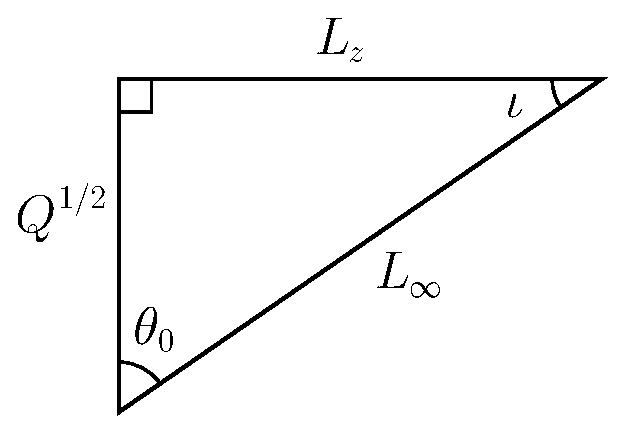
\includegraphics[width=0.35\textwidth]{./Images/Triangle.eps}
    \caption{The angular momenta $L_\infty$, $L_z$ and $\sqrt{Q}$ define a right-angled triangle. The acute angles are $\theta_0$, the extremal value of the polar angle, and $\iota$, the orbital inclination\cite{Glampedakis2002a}.}
   \label{fig:L_triangle}
\end{center}
\end{figure}
Let us now introduce a second angular variable\cite{Drasco2004}
\begin{equation}
\zeta = \zeta_0\cos^2\chi.
\end{equation}
Over one $2\pi$ period of $\chi$, $\theta$ oscillates over its full range, from its minimum value to its maximum and back. The geodesic equation for $\chi$ is
\begin{equation}
\rho^2\diff{\chi}{\tau} = \sqrt{Q + L_z^2},
\end{equation}
and may be integrated simply.

\section{Waveform Construction}

With the geodesic calculated for given angular momenta $L_z$ and $Q$, and initial starting positions, the orbiting body is assumed to follow this trajectory exactly: we ignore evolution due to the radiation of energy and angular momentum. From this we calculate the gravitational waveform using a semirelativistic approximation\cite{Ruffini1981}: we assume that the particle moves along a geodesic in the Kerr geometry, but radiates as if it were in flat spacetime. This quick-and-dirty technique is known as a numerical kludge\cite{Babak2007}.

\subsection{Kludge Approximation}

Numerical kludge approximations aim to encapsulate the main characteristics of a waveform by using the exact particle trajectory (ignoring inaccuracies from the evolution of the orbital parameters), whilst saving on computational time by using approximate waveform generation techniques. To start, we build an equivalent flat spacetime trajectory from the Kerr geodesic. This is done by identifying the Boyer-Lindquist coordinates with a set of flat-space coordinates; we consider two choices here:
\begin{enumerate}
\item Identify the Boyer-Lindquist coordinates with flat-space spherical polars \linebreak $\{r\sub{BL}, \theta\sub{BL}, \phi\sub{BL}\} \rightarrow \{r\sub{sph}, \theta\sub{sph}, \phi\sub{sph}\}$, then define flat-space Cartesian coordinates\cite{Gair2005, Babak2007}
\begin{equation}
\boldsymbol{x} = \left(r\sub{sph} \sin\theta\sub{sph}\cos\phi\sub{sph}, r\sub{sph} \sin\theta\sub{sph}\sin\phi\sub{sph}, r\sub{sph} \cos\theta\sub{sph}\right).
\end{equation}
\item Identify the Boyer-Lindquist coordinates with flat-space oblate-spheroidal coordinates $\{r\sub{BL}, \theta\sub{BL}, \phi\sub{BL}\} \rightarrow \{r\sub{ob}, \theta\sub{ob}, \phi\sub{ob}\}$ so that the flat-space Cartesian coordinates are
\begin{equation}
\boldsymbol{x} = \left(\sqrt{{r\sub{ob}}^2 + a^2} \sin\theta\sub{ob}\cos\phi\sub{ob}, \sqrt{{r\sub{ob}}^2 + a^2} \sin\theta\sub{ob}\sin\phi\sub{ob}, r\sub{ob} \cos\theta\sub{ob}\right).
\end{equation}
These are appealing because in the limit that $G \rightarrow 0$, so the gravitating mass goes to zero, the Kerr metric in Boyer-Lindquist coordinates reduces to the Minkowski metric in oblate spheroidal coordinates.%\footnote{We must take the limit $G \rightarrow 0$, rather than $M_\bullet \rightarrow 0$ to avoid the problem of an over-extreme BH with $a > M_\bullet$.}
\end{enumerate}
In the limit of $a \rightarrow 0$, the two coincide, as they do in the limit of large $r\sub{BL}$. It must be stressed that there is no well motivated argument that either coordinate system must yield an accurate GW; their use is justified {\it post facto} by comparison with result obtained from more accurate, and computationally intensive, methods\cite{Gair2005, Babak2007}. This ambiguity in assigning flat-space coordinates reflects the inconsistency of the semi-relativistic approximation: the geodesic trajectory was calculated for the Kerr geometry; by moving to flat spacetime we lose the reason for its existence. However, this inconsistency should not be regarded as a major problem; it is just an artifact of the basic assumption that the shape of the trajectory is important for determining the character of the radiation, but the curvature of the spacetime in the vicinity of the source is not. By binding the particle to the exact geodesic, we ensure that the kludge waveform has spectral components at the correct frequencies, but by assuming flat spacetime for generation of GWs they will not have the correct amplitudes.

\subsection{Quadrupole-Octopole Formula}

Now we have a flat-space particle trajectory $x\sub{p}^\mu(\tau)$, we may apply a flat-space wave generation formula. We shall use the quadrupole-octopole formula to calculate the gravitational strain\cite{Press1977, Bekenstein1973}
\begin{equation}
h^{jk}(t, \boldsymbol{x}) = -\frac{2G}{c^6r}\left[\ddot{I}^{jk} - 2n_i\ddot{S}^{ijk} + n_i\dddot{M}^{ijk}\right]_{t'/, =/, t - cr}
\label{eq:Octopole}
\end{equation}
where an overdot represents differentiation with respect to time $t$, $t'$ is the retarded time, $r = \left|\boldsymbol{x} - \boldsymbol{x}\sub{p}\right|$ is the radial distance, $\boldsymbol{n}$ is the radial unit vector, and the mass quadrupole ${I}^{jk}$, current quadrupole ${S}^{ijk}$ and mass octopole ${M}^{ijk}$ are defined by
\begin{align}
{I}^{jk}(t') = {} & \intd{}{}{{x'}^j{x'}^kT^{00}(t', \boldsymbol{x'})}{^3x'}\\
{S}^{ijk}(t') = {} & \intd{}{}{{x'}^j{x'}^kT^{0i}(t', \boldsymbol{x'})}{^3x'}\\
{M}^{ijk}(t') = {} & \recip{c}\intd{}{}{{x'}^i{x'}^j{x'}^kT^{00}(t', \boldsymbol{x'})}{^3x'}.
\end{align}
This is correct for a slow moving source. It is the familiar quadrupole formula\cite{Misner1973, Hobson2006}, derived from linearized theory, but with the next order term included. For a point mass the energy-momentum tensor $T^{\mu\nu}$ contains a $\delta$-function which allows easy evaluation of the integrals of the various moments to give
\begin{align}
{I}^{jk} = {} & c^2\mu x\sub{p}^jx\sub{p}^k\\
{S}^{ijk} = {} & c\mu v\sub{p}^ix\sub{p}^jx\sub{p}^k\\
{M}^{ijk} = {} & c\mu x\sub{p}^ix\sub{p}^jx\sub{p}^k.
\end{align}
To evaluate \eqnref{Octopole} we need up to the third time derivative of the position. The velocity $\boldsymbol{v}\sub{p} = \dot{\boldsymbol{x}}\sub{p}$ can be calculated from the geodesic equations: dividing by $\linediff{t}{\tau}$ gives $\dot{r}$, $\dot{\theta}$ and $\dot{\phi}$ which can then be transformed to the Cartesian velocities assuming either the spherical or oblate spheroidal coordinate system.\footnote{There is again the problem of the sign of the geodesic equations; this is simply solved by taking the sign as calculated by finite differencing the trajectory.} Expressions for the acceleration $\boldsymbol{a}\sub{p} = \ddot{\boldsymbol{x}}\sub{p}$ and the jerk $\boldsymbol{j}\sub{p} = \dddot{\boldsymbol{x}}\sub{p}$ are more involved, so these derivatives are found numerically using a simple difference formula to approximate the derivative as
\begin{equation}
\left.\diff{f}{t}\right|_{t_1} \approx \recip{2}\left[\frac{f(t_1) - f(t_0)}{t_1 - t_0} + \frac{f(t_2) - f(t_1)}{t_2 - t_1}\right],
\end{equation}
where $t_0$, $t_1$ and $t_2$ are subsequent (not necessarily uniformly spaced) time-steps.

Since we are only interested in GWs, we shall use the transverse-traceless (TT) gauge. The waveform is given in the TT gauge by\cite{Misner1973}
\begin{equation}
{h\super{TT}}_{jk} = P^l_jh_{lm}P^m_k - \recip{2}P_{jk}P^{lm}h_{lm},
\end{equation}
where the (spatial) projection operator $P_{ij}$ is
\begin{equation}
P_{ij} = \delta_{ij} - n_in_j.
\end{equation}

\section{Detection With LISA}

The LISA detector is a three-arm, space-borne laser interferometer\cite{Bender1998, Danzmann2003}. The three arms form an equilateral triangle that rotates as the system's centre of mass follows a circular, heliocentric orbit, trailing $\ang{20}$ behind the Earth. To describe the detector configuration, and to transform from the MBH coordinate system to those of the detector, we will find it useful to define three coordinate systems: those of the BH at the galactic centre $x_\bullet^i$; ecliptic coordinates centred at the solar system barycentre $x_\odot^i$, and coordinates that co-rotate with the detector $x\sub{d}^i$. The currently envisioned mission geometry is depicted in figures (??). The coordinate systems are related by a series of angles: $\Theta$ and $\Phi$ give the orientation of the solar system in the MBH's coordinates. These define the orientation of the MBH's spin axis $z_\bullet$. $\overline{\Theta}$ and $\overline{\Phi}$ give the position of the galactic centre in ecliptic coordinates. $\overline{\phi}$ gives LISA's orbital phase and $\varphi$ gives the rotational phase of the detector arms. Both of these vary linearly with time
\begin{equation}
\overline{\phi}(t) = \omega_\oplus t + \overline{\phi}_0; \quad \varphi(t) = -\omega_\oplus t + \varphi_0;
\end{equation}
where $\omega_\oplus$ corresponds to one rotation per year. Finally, $\alpha = \ang{60}$ is the inclination of the detector plane. We have computed the waveforms in the MBH's coordinates, however it is simplest to describe the measured signal using the detector's coordinates. To transform between coordinates we will use the matrix $A_{ij}$:
\begin{equation}
x\sub{d}^i = A^i_jx_\bullet^j; \quad h\sub{d}^{ij} = A^i_kA^j_lh_\bullet^{kl}.
\end{equation}
To define this, it is convenient to introduce angles
\begin{equation}
\Sigma = \overline{\Theta} + \Theta; \quad \delta = \overline{\phi} - \overline{\Phi}.
\end{equation}
The transformation matrix from the BH coordinates to the detector coordinates is
\begin{equation}
\left[A^i_j\right] = \begin{bmatrix}
a_{11} & a_{12} & a_{13} \\
a_{21} & a_{22} & a_{23} \\
a_{31} & a_{32} & a_{33}
\end{bmatrix};
\end{equation}
the elements are
\begin{align}
a_{11} = {} & s_\varphi\left(c_\delta s_\Phi - s_\delta c_\Phi c_\Sigma\right) - c_\varphi \left[s_\alpha c_\Phi s_\Sigma - c_\alpha \left(c_\delta c_\Phi c_\Sigma + s_\delta s_\Sigma\right)\right]; \\
a_{12} = {} & -s_\varphi\left(c_\delta c_\Phi - s_\delta s_\Phi c_\Sigma\right) - c_\varphi \left[s_\alpha s_\Phi s_\Sigma - c_\alpha \left(c_\delta s_\Phi c_\Sigma + s_\delta s_\Sigma\right)\right]; \\
a_{13} = {} & s_\varphi s_\delta s_\Sigma - c_\varphi\left(s_\alpha c_\Sigma + c_\alpha c_\delta s_\Sigma\right); \\
a_{21} = {} & s_\varphi\left[s_\alpha c_\Phi s_\Sigma - c_\alpha \left(c_\delta c_\Phi c_\Sigma + s_\delta s_\Sigma\right)\right] - c_\varphi \left(c_\delta s_\Phi - s_\delta c_\Phi s_\Sigma\right); \\
a_{22} = {} & s_\varphi\left[s_\alpha s_\Phi s_\Sigma - c_\alpha \left(c_\delta s_\Phi c_\Sigma + s_\delta s_\Sigma\right)\right] - c_\varphi \left(c_\delta c_\Phi - s_\delta s_\Phi s_\Sigma\right); \\
a_{23} = {} & s_\varphi\left(s_\alpha c_\Sigma + c_\alpha c_\delta s_\Sigma\right) - c_\varphi s_\delta s_\Sigma; \\
a_{31} = {} & -s_\alpha\left(c_\delta c_\Phi c_\Sigma + s_\delta s_\Phi\right) - c_\alpha c_\Phi s_\Sigma; \\
a_{32} = {} & s_\alpha\left(s_\delta c_\Phi - c_\delta s_\Phi c_\Sigma\right) - c_\alpha s_\Phi s_\Sigma; \\
a_{33} = {} & s_\alpha c_\delta s_\Sigma - c_\alpha c_\Sigma;
\end{align}
where we define $s_\vartheta \equiv \sin \vartheta$ and $c_\vartheta \equiv \cos \vartheta$.

The strains measured in the three arms can be combined such that LISA behaves as a pair of $\ang{90}$ interferometers at $\ang{45}$ to each other (with signals scaled by $\nicefrac{\sqrt{3}}{2}$)\cite{Cutler1998}. We will denote the two detectors as I and II. If we label the change in the three arms lengths caused by GWs $\delta L_1$, $\delta L_2$ and $\delta L_3$, and use $L$ for the unstrained length, then detector I measures strain
\begin{align}
h\sub{I}(t) = {} & \frac{\delta L_1 - \delta L_2}{L} \\
 = {} & \frac{\sqrt{3}}{2}\left(\recip{2} h\sub{d}^{xx} - \recip{2}h\sub{d}^{yy}\right),
\end{align}
and detector II measures
\begin{align}
h\sub{II}(t) = {} & \frac{\delta L_1 + \delta L_2 - 2 \delta L_3}{\sqrt{3}L} \\
 = {} & \frac{\sqrt{3}}{2}\left(\recip{2} h\sub{d}^{xy} + \recip{2} h\sub{d}^{yx}\right).
\end{align}
We will use vector notation $\boldsymbol{h}(t) = \left(h\sub{I}(t), h\sub{II}(t)\right) = \left\{h_A(t)\right\}$ to represent signals from both detectors.

The final consideration for calculating the signal measured by LISA is the time of arrival of the signal: LISA's orbital position changes with time. Fortunately over the timescales of interest for parabolic encounters, these changes are small. We will assume that the position of the solar system barycentre relative to the galactic centre is constant, at least over these short timescales: it is defined by the distance $R_0$ and the angles $\overline{\Theta}$ and $\overline{\Phi}$. The time of arrival at the solar system barycentre $t_\odot$ is then the appropriate retarded time. The time of detection $t\sub{d}$ to lowest order is then
\begin{equation}
t\sub{d} \simeq t_\odot - t\sub{AU}\cos\left[\overline{\phi}(t_\odot) - \overline{\Phi}\right]\sin\overline{\Theta},
\end{equation}
where $t\sub{AU}$ is the light travel-time for LISA's orbital radius. The time $t\sub{d}$ must be used for $\phi(t)$ and $\varphi(t)$.

\section{Signal Analysis}

\subsection{Frequency Domain Formalism}

At this stage we now know the GW $\boldsymbol{h}(t)$ that will be incident upon the LISA detector. We must now discuss how to analyse the waveform to extract the information it contains. We begin with a brief overview of the basic components of signal analysis used for GWs, with application to LISA in particular. This fixes the notation we will employ. A more complete discussion of material presented here can be found in the work of Finn\cite{Finn1992}, and Cutler and Flanagan\cite{Cutler1994}.

The actual measured strain $\boldsymbol{s}(t)$ will be the combination of the signal and the detector noise
\begin{equation}
\boldsymbol{s}(t) = \boldsymbol{h}(t) + \boldsymbol{n}(t),
\end{equation}
we will assume that the noise $n_A(t)$ is stationary and Gaussian. When analysing signals, it is most convenient to work with the Fourier transform
\begin{equation}
\tilde{g}(f) = \intd{-\infty}{\infty}{g(t)e^{2\pi i ft}}{t}.
\end{equation}
Since we have assumed Gaussianity for the noise signal $n_A(t)$, each Fourier component $\tilde{n}_A(f)$ also has a Gaussian probability distribution; the assumption of stationarity means that different Fourier components are uncorrelated, thus\cite{Cutler1994}
\begin{equation}
\left\langle\tilde{n}_A(f)\tilde{n}_B^*(f')\right\rangle_n = \recip{2}\delta(f - f')S_{AB}(f),
\end{equation}
where $\left\langle\ldots\right\rangle_n$ denotes the expectation value over the noise distribution, and $S_{AB}(f)$ is the (single-sided) noise spectral density. For simplicity, we may assume that the noise in the two detectors is uncorrelated, but share the same characterization so that\cite{Cutler1998}
\begin{equation}
S_{AB}(f) = \delta_{AB}S_n(f).
\end{equation}
The functional form of the noise spectral density $S_n(f)$ for LISA is discussed below in \secref{Noise}.

The properties of the noise allow us to define a natural inner product and associated distance on the space of signals\cite{Cutler1994}
\begin{equation}
\innerprod{\boldsymbol{g}}{\boldsymbol{k}} = 2\intd{0}{\infty}{\frac{\tilde{g}_A^*(f)\tilde{k}_A(f) + \tilde{g}_A(f)\tilde{k}_A^*(f)}{S_n(f)}}{f}.
\end{equation}
Using this definition, the probability of a particular realization of noise $\boldsymbol{n}(t) = \boldsymbol{n}_0(t)$ is
\begin{equation}
p(\boldsymbol{n}(t) = \boldsymbol{n}_0(t)) \propto \exp\left[-\recip{2}\innerprod{\boldsymbol{n}_0}{\boldsymbol{n}_0}\right].
\end{equation}
Thus, if the incident waveform is given as $\boldsymbol{h}(t)$, the probability of measuring signal $\boldsymbol{s}(t)$ is
\begin{equation}
p(\boldsymbol{s}(t)|\boldsymbol{h}(t)) \propto \exp\left[-\recip{2}\innerprod{\boldsymbol{s}-\boldsymbol{h}}{\boldsymbol{s}-\boldsymbol{h}}\right].
\label{eq:sig_prob}
\end{equation}

\subsection{LISA Noise Curve}\label{sec:Noise}

LISA's noise has two sources: instrumental noise and confusion noise, primarily from white dwarf binaries. The latter may be divided into contributions from galactic and extragalactic binaries. In this work we use the noise model of Barack and Cutler\cite{Barack2004}. The shape of the noise curve can be seen in figures (??). The instrumentation noise dominates at both high and low frequencies. The confusion noise is important at intermediate frequencies, and is responsible for the cusp around $f = \SI{1e-3}{\Hz}$.

\subsection{Window Functions}

There is one remaining complication regarding signal analysis. When we perform a Fourier transform using a computer we must necessarily only transform a finite time-span (it is a discrete Fourier transform).\footnote{The time-span in this case is the length of time the trajectory was calculated for.} The effect of this is the same as transforming the true, infinite signal multiplied by a unit top hat function of width equal to the time-span. Fourier transforming this yields the true waveform convolved with a sinc. If $\tilde{h}'(f)$ is the computed Fourier transform then
\begin{align}
\tilde{h}'(f) = {} & \intd{0}{\tau}{h(t)e^{2\pi i ft}}{t} \\
 = {} & \left[\tilde{h}(f) \ast e^{-\pi if\tau}\tau \sinc(\pi f\tau)\right],
\end{align}
where $\tilde{h}(f) = \mathscr{F}\{h(t)\}$, is the unwindowed Fourier transform. This windowing of the data is an inherent problem in the method; it will be as much of a problem when analysing signals from LISA as it is computing waveforms here. Windowing causes spectral leakage, which means that a contribution from large amplitude spectral components leaks into other components (side lobes), obscuring and distorting the spectrum at these frequencies\cite{Jones1982}.

Figure (??) shows the computed Fourier transforms for an example parabolic encounter. The waveforms have two distinct regions: a low-frequency curve, and a high-frequency tail. The low-frequency signal is the spectrum we are interested in; the high-frequency components are the result of spectral leakage. The $\order{\nicerecip{f}}$ behaviour of the sinc gives the shape of the tail. This has possibly been misidentified by Burko and Khanna\cite{Burko2007} as the characteristic strain for parabolic encounters.

Despite being many orders of magnitude below the peak level, the high-frequency tail is still well above the noise curve for a wide range of frequencies. It will therefore contribute to the evaluation of any inner products, and may mask interesting features. Unfortunately this is a fundamental problem that cannot be resolved completely. However, it is possible to the reduce the amount of spectral leakage using apodization: to improve the frequency response of a finite time series one can use a number of weighting window functions $w(t)$ which modify the impulse response in a prescribed way. The simplest window function is the rectangular (or Dirichlet) window; this is just the top hat described above. Other window functions are generally tapered. The introduction of a window function influences the spectrum in a manner dependent upon its precise shape; there are two distinct distortions: local smearing due to the finite width of the centre lobe, and distant leakage due to finite amplitude side lobes. Choosing a window-function is a trade-off between these two sources of error.

\section{Parameter Estimation}

Having detected a GW signal $\boldsymbol{s}(t)$ we are interested in what we may infer about the source. Let us define $\boldsymbol{\lambda} = \{\lambda^1, \lambda^2, \ldots, \lambda^N\}$ as the set of $N$ parameters which define the GW. We have an inference problem that may be solved by appropriate application of Bayes' Theorem\cite{Jaynes2003}: the probability distribution for our parameters given that we have detected the signal $\boldsymbol{s}(t)$ is given by the posterior
\begin{equation}
p(\boldsymbol{\lambda}|\boldsymbol{s}(t)) = \frac{p(\boldsymbol{s}(t)|\boldsymbol{\lambda})p(\boldsymbol{\lambda})}{p(\boldsymbol{s}(t))}.
\end{equation}
Here $p(\boldsymbol{s}(t)|\boldsymbol{\lambda})$ is the likelihood of the parameters, $p(\boldsymbol{\lambda})$ is the prior probability distribution for the parameters, and $p(\boldsymbol{s}(t)) = \intd{}{}{p(\boldsymbol{s}(t)|\boldsymbol{\lambda})}{^N \lambda}$ is, for our purposes a normalising constant, and may be ignored. The likelihood function depends upon the particular realization of noise. A particular set of parameters $\boldsymbol{\lambda}_0$ defines a waveform $\boldsymbol{h}_0(t) = \boldsymbol{h}(t; \boldsymbol{\lambda}_0)$, the probability that we observe signal $\boldsymbol{s}(t)$ for this GW is given by \eqnref{sig_prob}, so the likelihood is just
\begin{equation}
p(\boldsymbol{s}(t)|\boldsymbol{\lambda}_0) \propto \exp\left[-\recip{2}\innerprod{\boldsymbol{s}-\boldsymbol{h}_0}{\boldsymbol{s}-\boldsymbol{h}_0}\right].
\end{equation}
If we were to define this as a probability distribution for the parameters $\boldsymbol{\lambda}$, then the modal values would be the maximum-likelihood parameters $\boldsymbol{\lambda}\sub{ML}$. The waveform $h(t; \boldsymbol{\lambda}\sub{ML})$ would be the signal closest to $\boldsymbol{s}(t)$ in the space of all signal, where distance is defined using the inner product\cite{Cutler1994}.

In the limit of a high signal-to-noise ratio (SNR), we may approximate this as\cite{Vallisneri2008}
\begin{equation}
p(\boldsymbol{s}(t)|\boldsymbol{\lambda}_0) \propto \exp\left[-\recip{2}\innerprod{\partial_a\boldsymbol{h}}{\partial_b\boldsymbol{h}}\left(\lambda^a - \langle\lambda^a\rangle_\ell\right)\left(\lambda^b - \langle\lambda^b\rangle_\ell\right)\right],
\end{equation}
where the mean is defined as
\begin{equation}
\langle\lambda^a\rangle_\ell = \frac{\intd{}{}{\lambda^a p(\boldsymbol{s}(t)|\boldsymbol{\lambda})}{^N \lambda}}{\intd{}{}{p(\boldsymbol{s}(t)|\boldsymbol{\lambda})}{^N \lambda}}.
\end{equation}
Using the high SNR limit approximation, this mean is just the maximum-likelihood value $\langle\lambda^a\rangle_\ell = \lambda^a\sub{ML}$. The quantity
\begin{equation}
\Gamma_{ab} = \innerprod{\partial_a\boldsymbol{h}}{\partial_b\boldsymbol{h}}
\end{equation}
is the Fisher information matrix. We see that it controls the variance of likelihood distribution.

The form of the posterior distribution will depend upon the nature of the prior information. If we have an uninformative prior, such that $p(\boldsymbol{\lambda})$ is a constant, then the posterior distribution would be determined by the likelihood. In the high SNR limit, we would obtain a Gaussian with variance-covariance matrix
\begin{equation}
\boldsymbol{\Sigma} = \boldsymbol{\Gamma}^{-1}.
\end{equation}
The Fisher information matrix gives the uncertainty associated with the estimated parameter values, in this case the maximum-likelihood values. If the prior were to restrict the allowed range of parameters, for example, we believe that the spin parameter is $|a| \leq M_\bullet$; then the posterior would be a truncated Gaussian, and $\boldsymbol{\Gamma}^{-1}$ would no longer represent the variance-covariance. If the prior was approximately Gaussian with variance-covariance matrix $\boldsymbol{\Sigma}_0$, then the posterior would also be Gaussian.\footnote{If we only know the typical value and spread of a parameter then a Gaussian is the maximum entropy prior\cite{Jaynes2003}: the prior that is least informative given what we do know, the prior that best reflects our state of ignorance.} The posterior variance-covariance would be\cite{Cutler1994, Vallisneri2008}
\begin{equation}
\boldsymbol{\Sigma} = \left(\boldsymbol{\Gamma} + \boldsymbol{\Sigma}_0^{-1}\right)^{-1}.
\end{equation}

As a first estimate of what we may learn from parabolic encounters we have only looked at the Fisher information matrix elements. If these are large then we expect we would be able to precisely determine a parameter, whereas if they are small we would not be able to learn much more than we already believe from our prior knowledge. The input parameters for the model are:

\section{Energy Spectra}

We may compare the energy spectrum calculated from the kludge waveform with that obtained from the classic treatment of Peters and Matthews\cite{Peters1963, Peters1964}. These calculate GW emission for Keplerian orbits in flat spacetime, assuming only quadrupole radiation. The spectrum produced should be similar to that obtained from the NK in weak fields, that is for orbits with a large periapsis; however we do not expect an exact match because of the differing input physics and various approximations.

\subsection{Kludge Spectrum}

Our gravitational wave in the TT gauge has momentum pseudotensor\cite{Misner1973}
\begin{equation}
T_{\mu\nu} = \frac{c^4}{32\pi G}\left\langle\partial_\mu h_{ij} \partial_\nu h^{ij}\right\rangle,
\end{equation}
where $\langle\ldots\rangle$ indicates averaging over several wavelengths, or equivalently averaging over several periods. Thus, the flux of energy through a sphere of radius $r = R$ is
\begin{equation}
\diff{E}{t} = \frac{c^3}{32\pi G} R^2 \int{\dd\Omega}\left\langle\diff{h_{ij}}{t}\diff{h^{ij}}{t}\right\rangle,
\end{equation}
with $\intd{}{}{}{\Omega}$ representing integration over all solid angles. From \eqnref{Octopole} we see that the waves have a $\nicerecip{r}$ dependence, so if we define
\begin{equation}
h_{ij} = \frac{H_{ij}}{r},
\end{equation}
we see that the flux is independent of $R$, as required for energy conservation,
\begin{equation}
\diff{E}{t} = \frac{c^3}{32\pi G} \int{\dd\Omega}\left\langle\diff{H_{ij}}{t}\diff{H^{ij}}{t}\right\rangle.
\end{equation}
If we now integrate to find the total energy emitted we obtain
\begin{equation}
E = \frac{c^3}{32\pi G} \int{\dd\Omega}\int_{-\infty}^{\infty}{\dd t} \, \diff{H_{ij}}{t}\diff{H^{ij}}{t}.
\end{equation}
Since we are considering all time, the localization of the energy is no longer of importance and so it is unnecessary to average over several periods. If we switch to Fourier representation $\widetilde{H}_{ij}(f) = \mathscr{F}\{H_{ij}(t)\}$, then
\begin{align}
E = {} & \frac{c^3}{32\pi G} \int{\dd\Omega}\int_{-\infty}^{\infty}{\dd t}\intd{-\infty}{\infty}{}{f} \, 2\pi i f \widetilde{H}_{ij}(f)e^{2\pi i f t}\int_{-\infty}^{\infty}{\dd f'} \, 2\pi i f' \widetilde{H}^{ij}(f')e^{2\pi i f' t} \nonumber \\
 = {} & \frac{\pi c^3}{8 G} \int{\dd\Omega}\int_{-\infty}^{\infty}{\dd f} \, f^2 \widetilde{H}_{ij}(f)\widetilde{H}^{ij}(-f) \nonumber \\
 = {} & \frac{\pi c^3}{4 G} \int{\dd\Omega}\int_{0}^{\infty}{\dd f} \, f^2 \widetilde{H}^{ij}(f)\widetilde{H}_{ij}^*(f).
\end{align}
Here we have used that the signal is real so that $\widetilde{H}_{ij}^*(f) = \widetilde{H}_{ij}(-f)$. Using this we can identify the energy spectrum as
\begin{align}
\diff{E}{f} = \frac{\pi c^3}{4 G} \intd{}{}{}{\Omega} \, f^2 \widetilde{H}^{ij}(f)\widetilde{H}_{ij}^*(f).
\end{align}

\subsection{Peters \& Matthews Spectrum}

To calculate the energy spectrum for a parabolic orbit, we follow the derivation of Gair\cite{Gair2010}. Peters and Matthews give the power radiated into the $n$th harmonic of the orbital angular frequency as
\begin{equation}
P(n) = \frac{32}{5}\frac{G^4}{c^5}\frac{M_\bullet^2\mu^2(M_\bullet + \mu)(1-e)^5}{{r_p}^5}g(n,e)
\label{eq:PM_P}
\end{equation}
where the function $g(n,e)$ is defined in terms of Bessel functions of the first kind
\begin{align}
g(n,e) = {} & \frac{n^4}{32}\left\{\left[J_{n-2}(ne) - 2eJ_{n-1}(ne) + \frac{2}{n}J_n(ne) + 2eJ_{n+1}(ne) - J_{n+2}(ne)\right]^2 \right. \nonumber \\
 & + \left. \left(1 - e^2\right)\left[J_{n-2}(ne) - 2J_n(ne) + J_{n+2}(ne)\right]^2 + \frac{4}{3n^2}\left[J_n(ne)\right]^2\right\}.
\end{align}
The Keplerian orbital frequency is
\begin{align}
{\omega_0}^2 = {} & \frac{G(M_\bullet + \mu)(1-e)^3}{{r_p}^3}\\
 = {} & (1-e)^3{\omega\sub{c}}^2,
\label{eq:Kepler_freq}
\end{align}
where $\omega\sub{c}$ is defined as the orbital angular frequency of a circular orbit of radius equal to $r_p$. The total energy radiated into the $n$th harmonic, that is at frequency $\omega_n = n\omega_0$, is the power multiplied by the orbital period
\begin{equation}
E(n) = \frac{2\pi}{\omega_0}P(n);
\label{eq:E(n)}
\end{equation}
as $e \rightarrow 1$ for a parabolic orbit, $\omega_0 \rightarrow 0$ so the orbital period becomes infinite. We may therefore identify the energy radiated per orbit with the total orbital energy radiated. Since the spacing of harmonics is $\Delta\omega = \omega_0$, we may identify the energy spectrum
\begin{equation}
\left.\diff{E}{\omega}\right|_{\omega_n}\omega_0 = E(n).
\end{equation}
Using the above relations, and changing to linear frequency $2\pi f = \omega$, we obtain
\begin{align}
\left.\diff{E}{f}\right|_{f_n} = {} & \frac{128\pi^2}{5}\frac{G^3}{c^5}\frac{M_\bullet^2\mu^2}{r_p^2}(1-e)^2g(n,e) \\
 = {} & \frac{4\pi^2}{5}\frac{G^3}{c^5}\frac{M_\bullet^2\mu^2}{r_p^2}\ell(n,e),
\label{eq:PM_spectrum}
\end{align}
where we have defined the function $\ell(n,e)$ in the last line. For a parabolic orbit, we now have to take the limit of $\ell(n,e)$ as $e \rightarrow 1$. For this we shall use a number of properties of Bessel functions, and will make frequent reference to Watson\cite{Watson1995}.

We shall simplify $\ell(n,e)$ using the recurrence formulae (Watson\cite{Watson1995} 2.12)
\begin{align}
J_{\nu-1}(z) + J_{\nu+1}(z) = {} & \frac{2\nu}{z}J_\nu(z)\\
J_{\nu-1}(z) - J_{\nu+1}(z) = {} & 2J'_\nu(z).
\end{align}
We shall also eliminate $n$ using
\begin{align}
n = {} & \frac{\omega_n}{\omega_0} \nonumber \\
= {} & (1-e)^{-3/2}\widetilde{f}.
\end{align}
where $\widetilde{f} = \omega_n/\omega\sub{c} = f_n/f\sub{c}$ is a dimensionless frequency. We begin by breaking $\ell$ into three parts
\begin{align}
\ell = {} & \underbrace{(1-e)^2n^4\left[J_{n-2} - 2eJ_{n-1} + \frac{2}{n}J_n + 2eJ_{n+1} - J_{n+2}\right]^2}_{\ell_1} \nonumber \\
  & + \underbrace{(1-e)^3(1+e)n^4\left[J_{n-2} - 2J_n + J_{n+2}\right]^2}_{\ell_2} + \underbrace{\frac{4(1-e)^2n^2}{3}\left[J_n\right]^2}_{\ell_3}.
\end{align}
We have suppressed the argument of the Bessel functions for brevity. Tackling each term of $\ell$ in turn we obtain
\begin{align}
\ell_1(\widetilde{f},e) = {} & \left[\frac{4(1+e)\widetilde{f}^2}{e}\frac{J'_n}{1-e} + 2\frac{e-2}{e}\widetilde{f}\frac{J_n}{(1-e)^{1/2}}\right]^2\\
\ell_2(\widetilde{f},e) = {} & 16(1+e)\left[\frac{(1+e)\widetilde{f}^2}{e^2}\frac{J_n}{(1-e)^{1/2}} - \widetilde{f}\frac{J'_n}{e}\right]^2\\
\ell_3(\widetilde{f},e) = {} & \frac{4\widetilde{f}^2}{3}\left[{J_n}{(1-e)^{1/2}}\right]^2.
\end{align}
To take the limit of these we need to find the limiting behaviour of Bessel functions. We shall define two new functions
\begin{equation}
A(\widetilde{f}) = \lim_{e\rightarrow 1}\left\{\frac{J_n}{(1-e)^{1/2}}\right\}; \quad B(\widetilde{f}) = \lim_{e\rightarrow 1}\left\{\frac{J'_n}{1-e}\right\}.
\end{equation}
To give a well defined energy spectrum, both of these must be finite. In this case we see that the second term in $\ell_2$ should go to zero.

The Bessel function has an integral representation
\begin{equation}
J_\nu(z) = \recip{\pi}\intd{0}{\pi}{\cos(\nu\theta - z\sin\theta)}{\theta},
\end{equation}
we want the limit of this for $\nu \rightarrow \infty$, $z \rightarrow \infty$, with $z \leq \nu$. We will use the stationary phase approximation to argue that the predominant contribution to the integral comes from when the argument of the cosine is approximately zero, that is for small $\theta$ (Watson\cite{Watson1995} 8.2, 8.43). In this case we have
\begin{align}
J_\nu(z) \sim {} & \recip{\pi}\intd{0}{\pi}{\cos\left(\nu\theta - z\theta + \frac{z}{6}\theta^3\right)}{\theta}\\
 \sim {} & \recip{\pi}\intd{0}{\infty}{\cos\left(\nu\theta - z\theta + \frac{z}{6}\theta^3\right)}{\theta};
\end{align}
this last expression is an Airy integral. The Airy integral has a standard from (Watson\cite{Watson1995} 6.4)
\begin{equation}
\intd{0}{\infty}{\cos(t^3 + xt)}{t} = \frac{\sqrt{x}}{3}K_{1/3}\left(\frac{2x^{3/2}}{3^{3/2}}\right),
\end{equation}
where $K_\nu(z)$ is a modified Bessel function of the second kind. Using this to evaluate our limit gives
\begin{equation}
J_\nu(z) \sim \recip{\pi}\sqrt{\frac{2(\nu - z)}{3z}}K_{1/3}\left(\frac{2^{3/2}}{3}\sqrt{\frac{(\nu -z)^3}{z}}\right).
\end{equation}
For our particular case we have
\begin{equation}
\nu = (1 - e)^{-3/2}\widetilde{f}; \quad z = (1 - e)^{-3/2}e\widetilde{f};
\end{equation}
\begin{equation}
\frac{\nu - z}{z} = (1 - e); \quad \frac{(\nu - z)^3}{z} = \widetilde{f}^2;
\end{equation}
so we find
\begin{equation}
J_n(ne) \sim \recip{\pi}\sqrt{\frac{2}{3}}(1-e)^{1/2}K_{1/3}\left(\frac{2^{3/2}\widetilde{f}}{3}\right),
\end{equation}
thus
\begin{equation}
A(\widetilde{f}) = \recip{\pi}\sqrt{\frac{2}{3}}K_{1/3}\left(\frac{2^{3/2}\widetilde{f}}{3}\right)
\end{equation}
is well defined.

Now finding the derivative
\begin{align}
J'_\nu(z) = {} & \recip{2}\left[J_{\nu-1}(z) - J_{\nu+1}(z)\right] \nonumber \\
 \sim {} & \recip{2\pi}\left[\sqrt{\frac{2(\nu -1 - z)}{3z}}K_{1/3}\left(\frac{2^{3/2}}{3}\sqrt{\frac{(\nu - 1 - z)^3}{z}}\right) \right. \nonumber \\
  & \left. - \sqrt{\frac{2(\nu +1 - z)}{3z}}K_{1/3}\left(\frac{2^{3/2}}{3}\sqrt{\frac{(\nu + 1 - z)^3}{z}}\right)\right].
\end{align}
For our case
\begin{align}
\sqrt{\frac{\nu \pm 1 - z}{z}} = {} & (1 - e)^{1/2}\left[1 \pm \frac{(1-e)^{1/2}}{2\widetilde{f}} + \ldots\right];\\
\sqrt{\frac{(\nu \pm 1 - z)^{3/2}}{z}} = {} & \widetilde{f}\left[1 \pm \frac{3(1-e)^{1/2}}{2\widetilde{f}} + \ldots\right];
\end{align}
and so
\begin{align}
J'_n(ne) \sim {} & \recip{2\pi}\sqrt{\frac{2}{3}}(1-e)^{1/2}\left\{\left[1 - \frac{(1-e)^{1/2}}{2\widetilde{f}}\right]K_{1/3}\left(\frac{2^{3/2}\widetilde{f}}{3}\left[1 - \frac{3(1-e)^{1/2}}{2\widetilde{f}}\right]\right) \right. \nonumber \\
 & \left. - \left[1 + \frac{(1-e)^{1/2}}{2\widetilde{f}}\right]K_{1/3}\left(\frac{2^{3/2}\widetilde{f}}{3}\left[1 - \frac{3(1-e)^{1/2}}{2\widetilde{f}}\right]\right)\right]\nonumber \\
 \sim {} & \frac{-1}{2\pi}\sqrt{\frac{2}{3}}(1-e)\left[2^{3/2}K'_{1/3}\left(\frac{2^{3/2}\widetilde{f}}{3}\right) + \recip{\widetilde{f}}K_{1/3}\left(\frac{2^{3/2}\widetilde{f}}{3}\right)\right].
\end{align}
We may re-express the derivative using the recurrence formula (Watson\cite{Watson1995} 3.71)
\begin{equation}
K_{\nu-1}(z) - K_{\nu+1}(z) = -2K'_\nu(z)
\end{equation}
to give
\begin{equation}
J'_n(ne) \sim \frac{1-e}{\sqrt{3}\pi}\left[K_{-2/3}\left(\frac{2^{3/2}\widetilde{f}}{3}\right) + K_{4/3}\left(\frac{2^{3/2}\widetilde{f}}{3}\right) - \recip{\sqrt{2}\widetilde{f}}K_{1/3}\left(\frac{2^{3/2}\widetilde{f}}{3}\right)\right].
\end{equation}
And so finally,
\begin{equation}
B(\widetilde{f}) = \recip{\sqrt{3}\pi}\left[K_{-2/3}\left(\frac{2^{3/2}\widetilde{f}}{3}\right) + K_{4/3}\left(\frac{2^{3/2}\widetilde{f}}{3}\right) - \recip{\sqrt{2}\widetilde{f}}K_{1/3}\left(\frac{2^{3/2}\widetilde{f}}{3}\right)\right],
\end{equation}
which is also well defined.

Having obtained expressions for $A(\widetilde{f})$ and $B(\widetilde{f})$ in terms of standard functions, we may now calculate the energy spectrum for a parabolic orbit. From \eqnref{PM_spectrum} we have
\begin{equation}
\diff{E}{f} = \frac{4\pi^2}{5}\frac{G^3}{c^5}\frac{M_\bullet^2\mu^2}{r_p^2}\ell\left(\frac{f}{f\sub{c}}\right),
\label{eq:PM_dEdf}
\end{equation}
where we have used the limit
\begin{align}
\ell(\widetilde{f}) = {} & \lim_{e \rightarrow 1}\left\{\ell(n,e)\right\} \nonumber \\
 = {} & \left[8\widetilde{f}B(\widetilde{f}) - 2\widetilde{f}A(\widetilde{f})\right]^2 + \left(128\widetilde{f}^4 + \frac{4\widetilde{f}^2}{3}\right)\left[A(\widetilde{f})\right]^2.
\end{align}

To check the validity of this limit we may calculate the total energy radiated. We should be able to calculate this by integrating \eqnref{PM_dEdf} over all frequencies, or alternatively by summing the energy radiated into each harmonic. For consistency, the two approaches should yield the same result. First, summing over harmonics the
\begin{align}
E\sub{sum} = {} & \sum_n E(n) \nonumber \\
 = {} & \frac{64\pi}{5}\frac{G^3}{c^5}\frac{M_\bullet^2\mu^2}{r_p^2}\omega\sub{c}(1-e)^{7/2}\sum_n g(n,e),
\end{align}
where we have used equations \eqref{eq:PM_P}, \eqref{eq:Kepler_freq} and \eqref{eq:E(n)}. Peters and Matthews\cite{Peters1963} provide the result
\begin{equation}
\sum_n g(n,e) = \frac{1 + \nicefrac{73}{24}\, e^2 + \nicefrac{37}{96}\, e^4}{(1-e^2)^{7/2}}.
\end{equation}
Using this,
\begin{equation}
E\sub{sum} = \frac{64\pi}{5}\frac{G^3}{c^5}\frac{M_\bullet^2\mu^2}{r_p^2}\omega\sub{c}\frac{1 + \nicefrac{73}{24}\, e^2 + \nicefrac{37}{96}\, e^4}{(1+e^2)^{7/2}}.
\end{equation}
This is perfectly well behaved as $e \rightarrow 1$. Taking the limit for a parabolic orbit, the total energy radiated is
\begin{equation}
E\sub{sum} = \frac{85\pi}{2^{5/2}3}\frac{G^3}{c^5}\frac{M_\bullet^2\mu^2}{r_p^2}\omega\sub{c}.
\end{equation}
Integrating over the energy spectrum, \eqnref{PM_dEdf}, gives
\begin{align}
E\sub{int} = {} & \intd{0}{\infty}{\diff{E}{f}}{f} \nonumber \\
 = {} & \frac{2\pi}{5}\frac{G^3}{c^5}\frac{M_\bullet^2\mu^2}{r_p^2}\omega\sub{c}\intd{0}{\infty}{\ell(\widetilde{f})}{\widetilde{f}}.
\end{align}
The integral can be easily evaluated numerically showing
\begin{align}
\intd{0}{\infty}{\ell(\widetilde{f})}{\widetilde{f}} = {} & 12.5216858\ldots \nonumber \\
 = {} & \frac{425}{2^{7/2}3},
\end{align}
and so we find that the two total energies are consistent
\begin{align}
E\sub{int} = {} & \frac{85\pi}{2^{5/2}3}\frac{G^3}{c^5}\frac{M_\bullet^2\mu^2}{r_p^2}\omega\sub{c} \\
 = {} & E\sub{sum}.
\end{align}

\subsection{Comparison}


The total energy flux from the kludge waveform is larger than the Peters and Matthews result. This behaviour has been seen before for high eccentricity orbits about a non-spinning BH\cite{Gair2005}.

\section{Discussion \& Further Work}











\chapter{Future Work}

The work outlined in previous chapters should be largely completed by the end of 2010. It may be that further investigation reveals addition avenues to explore; however, it will be necessary to find new projects as well. Development of new areas of study will depend upon what is presented in the literature in the intervening time. Current ideas are discussed below.

\section{Other Theories Of Gravity}

Analysis similar to that discussed in chapter 1 for metric $f(R)$ gravity may be performed for other theories of modified gravity. This is a rapidly developing area incorporating ideas from quantum gravity and cosmology. Other theories to be investigated could include:
\begin{itemize}
\item Metric-affine gravity\cite{Sotiriou2007, Sotiriou2007b}, as discussed in \secref{Action}. Since this is not a metric theory of gravity it may be possible to find observational tests that strongly constrain, or rule out this theory\cite{Will2006}.
\item{} Generalised higher-order gravities which replace $R$ in the Einstein-Hilbert action with $f(R, R_{\mu\nu}R^{\mu\nu}, R_{\mu\nu\rho\sigma}R^{\mu\nu\rho\sigma})$\cite{Farhoudi2006, Madsen1989}. We see that $f(R)$ is just a simplification of this case. Again we should recover the results of quadratic gravity in linearized theory\cite{Pechlaner1966, Stelle1978, Schmidt1986, Teyssandier1990, Capozziello2009b}.
\item{} Ho\v{r}ava-Lifshitz gravity\cite{Horava2009, Blas2010a, Sotiriou2009c} which sacrifices spacetime covariance in favour of being renormalizable. A preferred foliation of space and time along the lines of the Arnowitt-Deser-Misner (ADM) formalism is adopted\cite{Arnowitt1962a}, with Lorentz invariance being emergent at large distances. This removes many of the problems associated with time traditionally associated with trying to quantize GR.
\end{itemize}
Since there are so many ways to formulate an alternate theory of gravity, there are many opportunities for study in this area. It would be desirable to find tests that can distinguish these theories from each other and GR, strong field tests seem the most promising.

\section{Observing Black Hole Shadows}

Black holes are intriguing objects objects. It the next few years it is hoped that very long baseline interferometry (VLBI) will advance to the stage that it will be possible resolve features of the order of the event horizon\cite{Doeleman2008}. This capability would allow us to directly image accretion flows down to the event horizon, and would be the first direct evidence that these compact object are actually black holes as currently understood, not some other exotic compact object.

One of the main targets of these strong field VLBI observations is the measurement of the BH's shadow. This is the dark region surrounding the BH from which no light can reach the observer; it is bounded by the inner most photon orbit\cite{Chandrasekhar1998}. The exact shape of the shadow is intimately linked to the metric and is a sensitive probe of the spacetime. By measuring the shape of the shadow it may be possible to measure the spin and inclination of the BH\cite{Hioki2009a}, assuming it is Kerr, check whether it is an over-extreme Kerr black hole\cite{Bambi2009}, or even probe deviations from Kerr\cite{Johannsen2010a, Johannsen2010b}. It would be interesting to investigate the shape of the shadow in other spacetimes, for example Manko-Novikov\cite{Manko1992, Gair2008a}. Observing deviations from Kerr would disprove the no hair theorem, possible admitting naked singularities, provide evidence for a non-GR theory of gravity, or both. In order to do so it will be necessary to find a convenient parameterization to describe the shape of the shadow.

\bibliographystyle{../physicsNEW}
\bibliography{../library}

\end{document}
